\documentclass[authoryear,review, 12pt]{elsarticle}



\newcommand{\maxwidth}{\textwidth}

\usepackage{alltt}
\usepackage[T1]{fontenc}
\usepackage[latin9]{inputenc}
\usepackage{geometry}
\geometry{verbose}
\setlength{\parskip}{\bigskipamount}
\setlength{\parindent}{0pt}
\usepackage{bm}
\usepackage{amsthm}
\usepackage{amsmath}
\usepackage{amssymb}
\usepackage{undertilde}
\usepackage{graphicx}
\usepackage{setspace}
\usepackage{esint}
\usepackage{booktabs}
\usepackage{color}
\usepackage{multirow}
\usepackage{natbib}

\mathchardef\mhyphen="2D % Define a "math hyphen"

\newcommand{\hlc}[2][yellow]{ {\sethlcolor{#1} \hl{#2}} }
\newcommand{\highlight}[1]{\colorbox{yellow}{$\displaystyle #1$}}

\newtheorem{thm}{Theorem}
\newtheorem{lem}{Lemma}

\newcommand\pr{\mathbf P}
\newcommand{\E}{\mathbb{E}}

\setlength{\textwidth}{6.5in}
\setlength{\textheight}{8.5in}
\textwidth=6.5in
\textheight=8.5in
\setlength{\topmargin}{0in}
\setlength{\oddsidemargin}{0in}
\setlength{\evensidemargin}{0in}

\journal{JRSSB}

\begin{document}


\begin{frontmatter}

\title{Local Adaptive Grouped Regularization and its Oracle Properties for Varying Coefficient Regression}


\author[wrbrooks]{Wesley Brooks}
\ead{wrbrooks@uwalumni.com}

\author[jzhu]{Jun Zhu}
\ead{jzhu@stat.wisc.edu}

\author[zlu]{Zudi Lu}
\ead{Z.Lu@soton.ac.uk}

\address[wrbrooks]{Department of Statistics, University of Wisconsin, Madison, WI 53706}
\address[jzhu]{Department of Statistics and Department of Entomology, University of Wisconsin, Madison, WI 53706}
\address[zlu]{School of Mathematical Sciences, The University of Southampton, Highfield, Southampton UK}

\begin{abstract}
Varying coefficient regression is a flexible technique for modeling data where the coefficients are functions of some effect-modifying parameter, often time or location. While there are a number of methods for variable selection in a varying coefficient regression model, the existing methods mostly do global selection, which includes or excludes each covariate over the entire domain. Presented here is a new local adaptive grouped regularization (LAGR) method for local variable selection in spatially varying coefficient linear and generalized linear regression. LAGR selects the covariates that are associated with the response at any point in space, and simultaneously estimates the coefficients of those covariates by tailoring the adaptive group Lasso toward a local regression model with locally linear coefficient estimates. Oracle properties of the proposed method are established under local linear regression and local generalized linear regression. The finite sample properties of LAGR are assessed in a simulation study and for illustration, the Boston housing price data set is analyzed.
\end{abstract}

\begin{keyword}
adaptive Lasso, local generalized linear regression, local linear regression, regularization method, nonparametric, varying coefficient model
\end{keyword}

\end{frontmatter}

\section{Introduction}

Whereas the coefficients in traditional linear regression are scalar
constants, the coefficients in a varying coefficient regression (VCR)
model are functions - often \emph{smooth} functions - of some effect-modifying
parameter \citep{Cleveland-Grosse-1991,Hastie-Tibshirani-1993}. Here
we treat the case of a VCR model on a spatial domain where the spatial
location is a two-dimensional effect-modifying parameter. Current
practice for VCR models relies on global model selection to decide
which variables should be included in the model, meaning that covariates
are selected for inclusion or exclusion over the entire spatial domain.
Various methods have been developed by using, for example, P-splines
\citep{Antoniadis:2012a}, basis expansion \citep{Wang-2008a}, and
local regression \citep{Wang-Xia-2009}. Since the coefficients vary
in a VCR model, in principle there is no reason that the best model
must use the same set of covariates everywhere on the domain - that
is, some of the coefficients may be zero in part of the domain. New
methodology is developed here for guiding the decision of which covariates
belong in the VCR model at any location, or local variable selection,
as the literature on how to do so is currently scarce.

Specifically, local adaptive grouped regularization (LAGR) is developed
here as a method of local variable selection at any given location
in the domain of a VCR model. The method of LAGR applies to VCR models
where the coefficients are estimated using locally linear kernel smoothing.
Kernel smoothing for nonparametric regression is described in detail
in \citet*{Fan-Gijbels-1996}. The extension to estimating VCR models
is made by \citet{Fan-Zhang-1999} for a VCR model with a univariate
effect-modifying parameter, and by \citet{Sun-Yan-Zhang-Lu-2014}
for a two-dimensional effect-modifying parameter in a spatial VCR
with autocorrelation. These methods mitigate the boundary effect by
estimating the coefficients as local polynomials of odd degree (usually
locally linear) \citep{Hastie:1993b}. In this work, we focus on a
two-dimensional effect-modifying parameter and discuss the effect
of different dimensionality on the results.

For standard linear regression models, the least absolute shrinkage
and selection operator (Lasso) is a penalized regression method that
simultaneously selects covariates for the regression model and shrinks
the coefficient estimates toward zero \citep{Tibshirani-1996}. However,
the Lasso can be inconsistent for variable selection and inefficient
for coefficient estimation \citep{Zou-2006}. The adaptive Lasso (AL)
is a refinement of the Lasso that produces consistent estimates of
the coefficients and has been shown to have appealing properties for
variable selection, which under suitable conditions include the ``oracle''
property of asymptotically including exactly the correct set of covariates
and estimating their coefficients as well as if the correct covariates
were known in advance \citep{Zou-2006}. For data where the observed
covariates fall into mutually exclusive groups that are known in advance,
the adaptive group Lasso has similar oracle properties to the adaptive
Lasso but does selection on groups rather than individual covariates
\citep{Yuan-Lin-2006,Wang-Leng-2008}. The main innovation of the
proposed LAGR method is to tailor the adaptive group Lasso toward
local variable selection and coefficient estimation in a locally linear
regression model, where each group consists of a single covariate
and its interactions with location. Further, we extend the method
from varying coefficient linear regression to varying coefficient
generalized linear regression for responses that are not necessarily
Gaussian. We show that LAGR possesses the oracle properties of asymptotically
selecting exactly the correct local covariates and estimating their
local coefficients as accurately as would be possible if the identity
of the nonzero coefficients for the local model were known in advance.

The remainder of this paper is organized as follows. The kernel-based
estimation of a VCR model is described in Section \ref{sec:vcr}.
The proposed LAGR technique for varying coefficient linear regression
and its oracle properties are presented in Section \ref{sec:lagr-gaussian}.
In Section \ref{sec:simulations}, the finite-sample properties of
LAGR are evaluated in a simulation study, and in Section \ref{sec:example}
LAGR is applied to the Boston housing price dataset. In Section \ref{sec:lagr-gllm},
LAGR is extended to varying coefficient generalized linear regression
and the oracle properties for this setting are established, followed
by conclusions and discussion in section 7. Technical proofs are left
to the appendices.

\section{Varying Coefficient Regression\label{sec:vcr}}

\subsection{Varying Coefficient Model}

Consider $n$ observation locations $\bm{s}_{i}=(s_{i,1},\; s_{i,2})^{T}$
for $i=1,\dots,n$, which are distributed in a domain $\mathcal{D}\subset\mathbb{R}^{2}$
according to a density $f$. For $i=1,\dots,n$, let $Y_{i}=Y(\bm{s}_{i})$
and $\bm{X}_{i}=\bm{X}(\bm{s}_{i})$ denote, respectively, the univariate
response and the $(p+1)$--vector of covariates measured at location
$\bm{s}_{i}$. At each location $\bm{s}_{i}$, assume that the outcome
is related to the covariates by a linear regression where the coefficients
$\bm{\beta}(\bm{s}_{i})$ are functions in the two dimensions and
$\varepsilon_{i}$ is random error at location $\bm{s}_{i}$. That
is, 
\begin{align}
Y_{i}=\bm{X}_{i}^{T}\bm{\beta}(\bm{s}_{i})+\varepsilon_{i}.\label{eq:lm(s)}
\end{align}

Further assume that the error term $\varepsilon_{i}$ is normally
distributed with zero mean and variance $\sigma^{2}$, and that $\varepsilon_{i}$,
$i=1,\dots,n$ are independent. That is, for $\bm{\varepsilon}=\left(\varepsilon_{1},\dots,\varepsilon_{n}\right)^{T}$,
$\bm{\varepsilon}\sim N\left(\bm{0},\sigma^{2}\bm{I}_{n}\right)$
where $\bm{I}_{n}$ denotes the identity matrix. 

In the context of nonparametric regression, the boundary-effect bias
can be reduced by local polynomial modeling, usually in the form of
a locally linear model \citep{Fan-Gijbels-1996}. Here, to prepare
for the estimation of locally linear coefficients, we augment the
design matrix and the coefficient surfaces with interactions on location in two dimensions
\citep{Wang-2008b}. Let $\bm{X}=\left(\bm{X}_{1},\dots,\bm{X}_{n}\right)^{T}$
be the design matrix of observed covariate values. Then the augmented
local design matrix at location $\bm{s}$ is defined to be $\bm{Z}(\bm{s})=\left(\bm{X}\ \:\bm{L}(\bm{s}) \bm{X}\ \:\bm{M}(\bm{s}) \bm{X}\right),$
where $\bm{L}(\bm{s})=\text{diag}\{s_{i',1}-s_1\}_{i'=1}^{n}$ and
$\bm{M}(\bm{s})=\text{diag}\{s_{i',2}-s_2\}_{i'=1}^{n}$. 
The vector of augmented local coefficients at location $\bm{s}$ is defined to be $\bm{\zeta}(\bm{s})=\left(\bm{\beta}(\bm{s})^{T},\;\nabla_{u}\bm{\beta}(\bm{s})^{T},\;\nabla_{v}\bm{\beta}(\bm{s})^{T}\right)^{T}$,
where $\nabla_{u}\bm{\beta}(\bm{s})$ and $\nabla_{v}\bm{\beta}(\bm{s})$ denote the local gradients 
of the coefficient surfaces.

\subsection{Coefficient Estimation via Local Likelihood}



%Now we have $Y_{i}=\bm{Z}_{i}^{T}\bm{\zeta}_{i}+\varepsilon_{i}$.

Let $\bm{\zeta}=\left(\bm{\zeta}(\bm{s}_{1}),\dots,\bm{\zeta}(\bm{s}_{n})\right)^{T}$
denote a matrix of the local coefficients at all observation locations
$\bm{s}_{1},\dots,\bm{s}_{n}$ and let $\left\{\bm{Z}(\bm{s})\right\}_{i}$ denote the
$i$th row of the matrix $\bm{Z}(\bm{s})$ as a column vector. The total log-likelihood of the observed
data is the sum of the log-likelihood of each individual observation:
\begin{align}
\ell\left(\bm{\zeta}\right)= & -(1/2)\sum_{i=1}^{n}\left[\log{\sigma^{2}}+\sigma^{-2}\left\{ y_{i}- \{\bm{z}(\bm{s}_i)\}_i \bm{\zeta}(\bm{s}_{i})\right\} ^{2}\right].\label{eq:coefficients}
\end{align}

Since there are a total of $3(p+1)n+1$ parameters for $n$ observations,
the model is not identifiable and it is not possible to directly maximize
the total likelihood. When the coefficient functions are smooth, though,
the coefficients $\bm{\zeta}(\bm{s})$ at location $\bm{s}$ can be
approximated by the coefficients $\bm{\zeta}(\bm{t})$ , where $\bm{t}$
is within some neighborhood of $\bm{s}$. This intuition is formalized
by the following local log-likelihood at location $\bm{s}\in\mathcal{D}$:
\begin{align}
\ell\left(\bm{\zeta}(\bm{s})\right)= & -(1/2)\sum_{i=1}^{n}K_{h}(\|\bm{s}-\bm{s}_{i}\|)\left[\log\sigma^{2}+\sigma^{-2}\left\{ y_{i}-\bm{z}_{i}^{T}\bm{\zeta}(\bm{s})\right\} ^{2}\right]\label{eq:local-log-likelihood}
\end{align}

where $\bm{Z}_{i}=\left\{\bm{Z}(\bm{s})\right\}_{i}$, $h$ is a bandwidth parameter, $\|\cdot\|$ is the $\ell_{2}$-norm,
and $K_{h}(\|\bm{s}-\bm{s}_{i}\|)$ for $i=1,\dots,n$ are local weights
from a kernel function. For instance, the Epanechnikov kernel is defined
as $K_{h}(\|\bm{s}_{i}-\bm{s}_{i'}\|)=h^{-2}K\left(h^{-1}\|\bm{s}_{i}-\bm{s}_{i'}\|\right)$
where $K(x)=(3/4)(1-x^{2})$ if $x<1$, and $0$ otherwise \citep{Samiuddin-el-Sayyad-1990}.

The local log-likelihood (\ref{eq:local-log-likelihood}) is maximized
to obtain an estimate $\tilde{\bm{\zeta}}(\bm{s})$ of the local coefficients
at $\bm{s}$. Let $\bm{W}\!(\bm{s})={\rm diag}\left\{ K_{h}(\|\bm{s}-\bm{s}_{i}\|)\right\} _{i'=1}^{n}$
denote a diagonal matrix of kernel weights. The local likelihood (\ref{eq:local-log-likelihood})
can be maximized by minimizing a locally weighted least squares: 
\begin{equation}
\mathcal{S}\left(\bm{\zeta}(\bm{s})\right)=(1/2)\left\{ \bm{Y}-\bm{Z}(\bm{s})\bm{\zeta}(\bm{s})\right\} ^{T}\bm{W}\!(\bm{s})\left\{ \bm{Y}-\bm{Z}(\bm{s})\bm{\zeta}(\bm{s})\right\} .\label{eq:local-sum-of-squares}
\end{equation}

The minimizer of (\ref{eq:local-sum-of-squares}) is
\begin{equation}
\tilde{\bm{\zeta}}(\bm{s})=\left\{ \bm{Z}(\bm{s})^{T}\bm{W}\!(\bm{s})\bm{Z}(\bm{s})\right\} ^{-1}\bm{Z}(\bm{s})^{T}\bm{W}\!(\bm{s})\bm{Y}.\label{eq:zeta-hat}
\end{equation}

By Theorem 3 of \citet{Sun-Yan-Zhang-Lu-2014}, for any given $\bm{s}$,
the estimated local coefficients $\tilde{\bm{\beta}}(\bm{s})=\left(\tilde{\zeta}_{1}(\bm{s}),\dots,\tilde{\zeta}_{p}(\bm{s})\right)^{T}$
converge in probability at the optimal rate of $O\left(n^{-1/3}\right)$
and are asymptotically normally distributed. The bias of the local
coefficient estimates is proportional to the second derivatives of
the true coefficient functions.

\section{Local Variable Selection with LAGR\label{sec:lagr-gaussian}}

\subsection{LAGR Penalized Local Likelihood}

Estimating the local coefficients by (\ref{eq:zeta-hat}) has traditionally
relied on variable selection \emph{a priori}; that is, a set of covariates
is pre-determined. Here we develop a new method of penalized regression
to simultaneously select covariates locally and estimate the corresponding
local coefficients. For this purpose, each raw covariate is grouped
with its covariate-by-location interactions. That is, $\bm{\zeta}_{(j)}(\bm{s})=\left(\beta_{j}(\bm{s}),\;\;\nabla_{u}\beta_{j}(\bm{s}),\;\;\nabla_{v}\beta_{j}(\bm{s})\right)^{T}$
for $j=1,\dots,p$. The proposed LAGR penalty is akin to the adaptive
group Lasso \citep{Yuan-Lin-2006,Wang-Leng-2008}. By the mechanism
of the adaptive group Lasso, covariates within the same group are
included in or dropped from the model together. The intercept group
is left unpenalized.

To select and estimate the local coefficients at location $\bm{s}$,
we minimize a penalized local sum of squares at location $\bm{s}$:
\begin{align}
\mathcal{J}\left(\bm{\zeta}(\bm{s})\right) & =\mathcal{S}\left(\bm{\zeta}(\bm{s})\right)+\mathcal{P}\left(\bm{\zeta}(\bm{s})\right),\label{eq:penalized-least-squares}
\end{align}

where $\mathcal{S}\left(\bm{\zeta}\left(\bm{s}\right)\right)$ is
the locally weighted least squares defined in (\ref{eq:local-sum-of-squares}),
$\mathcal{P}\left(\bm{\zeta}(\bm{s})\right)=\sum_{j=1}^{p}\phi_{j}(\bm{s})\|\bm{\zeta}_{(j)}(\bm{s})\|$
is a local adaptive grouped regularization (LAGR) penalty. The LAGR
penalty for the $j$th group of coefficients at location $\bm{s}$
is $\phi_{j}(\bm{s})=\lambda_{n}\|\tilde{\bm{\zeta}}_{(j)}(\bm{s})\|^{-\gamma}$,
where $\lambda_{n}>0$ is a local tuning parameter applied to all
coefficients at location $\bm{s}$, $\tilde{\bm{\zeta}}_{(j)}(\bm{s})$
is a the vector of unpenalized local coefficients for the $j$th covariate
and its interactions on location from (\ref{eq:zeta-hat}), and $\gamma>1$.

Minimization of (\ref{eq:penalized-least-squares}) is by blockwise
coordinate descent, where each block is a covariate group (one raw
covariate and its interactions on location). Software for estimating
$\bm{\zeta}(\bm{s})$ will be made available in an \texttt{R} package.

\subsection{Oracle Properties\label{sub:oracle-properties}}

At location $\bm{s}$, let there be are $p_{0}<p$ covariates $\bm{X}_{(a)}(\bm{s})$
with nonzero local regression coefficients, denoted $\bm{\beta}_{(a)}(\bm{s})\ne\bm{0}$.
Without loss of generality, assume the indices of these covariates
are $1,\dots,p_{0}$. The remaining $p-p_{0}$ covariates $\bm{X}_{(b)}(\bm{s})$
have coefficients equal to zero, denoted $\bm{\beta}_{(b)}(\bm{s})=\bm{0}$.
Denote by $a_{n}=\max\left\{ \phi_{j}(\bm{s}),j\le p_{0}\right\} $
the largest penalty applied to a covariate group whose true coefficient
norm is nonzero, and by $b_{n}=\min\left\{ \phi_{j}(\bm{s}),j>p_{0}\right\} $
the smallest penalty applied to a covariate group whose true coefficient
norm is zero. Let $\bm{Z}_{(k)}(\bm{s})$ be the augmented design
matrix for covariate group $k$, and let $\bm{Z}_{(\mhyphen k)}(\bm{s})$
be the augmented design matrix for all the data except covariate group
$k$. Similarly, let $\bm{\zeta}_{(k)}(\bm{s})$ be the augmented
coefficients for covariate group $k$ and $\bm{\zeta}_{(\mhyphen k)}(\bm{s})$
be the augmented coefficients for all covariate groups except $k$.
Let $\nabla\zeta_{j}(\bm{s})=\left(\nabla_{u}\zeta_{j}(\bm{s}),\nabla_{v}\zeta_{j}(\bm{s})\right)^{T}$
and $\nabla^{2}\zeta_{j}(\bm{s})=\left(\begin{array}{cc}
\nabla_{uu}^{2}\zeta_{j}(\bm{s}) & \nabla_{uv}^{2}\zeta_{j}(\bm{s})\\
\nabla_{vu}^{2}\zeta_{j}(\bm{s}) & \nabla_{vv}^{2}\zeta_{j}(\bm{s})
\end{array}\right)$. Let $\kappa_{0}=\int_{\mathbb{R}^{2}}K(\|\bm{s}\|)d\bm{s}$, $\kappa_{2}=\int_{\mathbb{R}^{2}}[(1,0)\bm{s}]^{2}K(\|\bm{s}\|)d\bm{s}=\int_{\mathbb{R}^{2}}[(0,1)\bm{s}]^{2}K(\|\bm{s}\|)d\bm{s}$,
and $\nu_{0}=\int_{\mathbb{R}^{2}}K^{2}(\|\bm{s}\|)d\bm{s}$. Finally,
let $\xrightarrow{p}$ and $\xrightarrow{d}$ denote convergence in
probability and distribution, respectively, as $n\to\infty$.

Assume the following regularity conditions.
\begin{itemize}
\item[(C.1)] The kernel function $K(\cdot)$ is bounded, positive, symmetric,
and Lipschitz continuous on $\mathbb{R}$, and has a bounded support.
\item[(C.2)] The coefficient functions $ $$\beta_{j}(\cdot)$ for $j=1,\dots,p$
have continuous second-order partial derivatives at $\bm{s}$.
\item[(C.3)] The covariates $\bm{X}(\bm{s}_{1}),\dots,\bm{X}(\bm{s}_{n})$ are
random vectors that are independent of $\varepsilon_{1},\dots,\varepsilon_{n}$.
Also $\bm{\Psi}(\bm{s})=E\left\{ \bm{X}(\bm{s})\bm{X}(\bm{s})^{T}|\bm{s}\right\} $
and $\bm{\Psi}_{(a)}(\bm{s})=E\left\{ \bm{X}_{(a)}(\bm{s})\bm{X}_{(a)}(\bm{s})^{T}|\bm{s}\right\} $
are positive-definite and differentiable at location $\bm{s}$.
\item[(C.4)] $E\left\{ \left|\bm{X}(\bm{s})\right|^{3}|\bm{s}\right\} $ and $E\left\{ Y(\bm{s})^{4}|\bm{X}(\bm{s}),\bm{s}\right\} $
are continuous at a given location $\bm{s}$.
\item[(C.5)] The observation locations $\{\bm{s}_{i}\}$ are a sequence of fixed
design points on a bounded compact support $\mathcal{S}$. Further,
there exists a positive joint density function $f(\cdot)$ satisfying
a Lipschitz condition such that 
\[
\sup_{\bm{s}\text{\ensuremath{\in}}\mathcal{S}}\left|n^{-1}\sum_{i=1}^{n}\left[r(\bm{s}_{i})K_{h}(\|\bm{s}_{i}-\bm{s}\|)\right]-\int r(\bm{t})K_{h}(\|\bm{t}-\bm{s}\|)f(\bm{t})d\bm{t}\right|=O(h)
\]
where $f(\cdot)$ is bounded away from zero on $\mathcal{S}$, $r(\cdot)$
is any bounded continuous function, and $K_{h}(\cdot)=K(\cdot/h)/h^{2}$.
\item[(C.6)] $h=O\left(n^{-1/6}\right)$.
\item[(C.7)] $h^{-1}n^{-1/2}a_{n}\xrightarrow{p}0$ and $hn^{-1/2}b_{n}\xrightarrow{p}\infty$.
\end{itemize}
Conditions (C.1)--(C.4) are common in the literature on nonparametric
estimation, for instance see conditions (1)--(3) of \citet{Sun-Yan-Zhang-Lu-2014}
and conditions (5) and (6) of \citet{Cai-Fan-Li-2000}. However, the
covariates $\bm{X}(\bm{s}_{1}),\dots,\bm{X}(\bm{s}_{n})$ were assumed
to be $iid$ in \citet{Sun-Yan-Zhang-Lu-2014}, which is not required
here. The existence of of $\bm{\Psi}(\cdot)$ is needed for the existence
of the limiting distribution of $\hat{\bm{\beta}}(\bm{s})$; its differentiability
is used in the Taylor's expansions. Condition (C.4) is used when bounding
the remainder term in the Taylor's expansions. Condition (C.5) is
the same as condition (4) of \citet{Sun-Yan-Zhang-Lu-2014}, which
is more general than strict infill asymptotics, as in the latter case
the elements of $\{\bm{s}_{i}\}$ are $iid$ as density $f(\cdot)$,
and the Lipschitz condition in (C.5) is satisfied with probability
one. Under condition (C.6), the coefficient estimates attain the optimal
rate of convergence for bivariate nonparametric regression. Condition
(C.7) is needed for establishing the oracle properties, and is a refinement
of the condition for the adaptive group lasso \citep{Wang-Leng-2008}.
In particular, satisfying (C.7) requires an additional restriction
on $\gamma$, the unpenalized group norm exponent in the LAGR penalty.

Under condition (C.7), the local penalty tends to zero on covariates
with true nonzero coefficients and to infinity on covariates with
true zero coefficients. By (C.7), $h^{-1}n^{-1/2}\lambda_{n}\to0$
for all $j\le p_{0}$ and $hn^{-1/2}\lambda_{n}\|\bm{\zeta}_{(j)}(\bm{s})\|^{-\gamma}\to\infty$
for all $j>p_{0}$. We require that $\lambda_{n}$ satisfy both assumptions.
Suppose $\lambda_{n}=n^{\alpha}$. Since $h=O\left(n^{-1/6}\right)$
and $\|\tilde{\bm{\zeta}}_{(p)}(\bm{s})\|=O\left(h^{-1}n^{-1/2}\right)$,
it follows that $h^{-1}n^{-1/2}\lambda_{n}=O\left(n^{-1/3+\alpha}\right)$
and $hn^{-1/2}\lambda_{n}\|\tilde{\bm{\zeta}}_{(p)}(\bm{s})\|^{-\gamma}=O\left(n^{-2/3+\alpha+\gamma/3}\right)$.
Thus, $\left(2-\gamma\right)/3<\alpha<1/3$, which can only be satisfied
for $\gamma>1$.
\begin{thm}[Asymptotic normality]
\label{theorem:normality}  Under (C.1)--(C.8),
\begin{gather*}
\left\{ f(\bm{s})h^{2}n\right\} ^{1/2}\left[\hat{\bm{\beta}}_{(a)}(\bm{s})-\bm{\beta}_{(a)}(\bm{s})-(2\kappa_{0})^{-1}\kappa_{2}h^{2}\left\{ \nabla_{uu}^{2}\bm{\beta}_{(a)}(\bm{s})+\nabla_{vv}^{2}\bm{\beta}_{(a)}(\bm{s})\right\} \right]\\
\xrightarrow{d}N\left(0,\kappa_{0}^{-2}\nu_{0}\sigma^{2}\Psi_{(a)}(\bm{s})^{-1}\right),
\end{gather*}
where $\left\{ \nabla_{uu}^{2}\bm{\beta}_{(a)}(\bm{s})+\nabla_{vv}^{2}\bm{\beta}_{(a)}(\bm{s})\right\} =\left(\nabla_{uu}^{2}\bm{\beta}_{1}(\bm{s})+\nabla_{vv}^{2}\bm{\beta}_{1}(\bm{s}),\dots,\nabla_{uu}^{2}\bm{\beta}_{p_{o}}(\bm{s})+\nabla_{vv}^{2}\bm{\beta}_{p_{o}}(\bm{s})\right)^{T}$.
\end{thm}

\begin{thm}[Selection consistency]
\label{theorem:selection} Under (C.1)--(C.8), 
\[
P\left\{ \|\hat{\bm{\zeta}}_{(j)}(\bm{s})\|=\bm{0}\right\} \to1\text{ if }j>p_{0}.
\]
\end{thm}
Theorem \ref{theorem:normality} indicates that the LAGR estimates
for true nonzero coefficients have the same asymptotic distribution
as a local regression model where the true nonzero coefficients are
known in advance. Further, by Theorem \ref{theorem:selection}, the
LAGR estimates of true zero coefficients tend to zero with probability
one. Together, selection and local coefficient estimation by LAGR
has the oracle property. The technical proofs of Theorems \ref{theorem:normality}
and \ref{theorem:selection} are given in Appendix A.

\subsection{Tuning Parameter Selection}

In practical application, it is necessary to select the LAGR tuning
parameter $\lambda_{n}$ for each local model. A popular approach
in other Lasso-type problems is to select the tuning parameter that
maximizes a criterion that approximates the expected log-likelihood
of a new, independent data set drawn from the same distribution. This
is the framework of Mallows' Cp, Stein's unbiased risk estimate (SURE)
and Akaike's information criterion (AIC) \citep{Mallows-1973,Stein-1981,Akaike-1973}.

These criteria use a so-called covariance penalty to estimate the
bias due to using the same data set to select a model and to estimate
its parameters \citep{Efron:2004a}. We adopt the approximate degrees
of freedom for the adaptive group Lasso from \citet{Yuan-Lin-2006}
and minimize the AICc to select the tuning parameter $\lambda_{n}$
\citep{Hurvich-1998}. That is, let

\begin{align*}
\hat{{\rm df}}(\lambda_{n};\bm{s})= & \sum_{j=1}^{p}I\left(\|\hat{\bm{\zeta}}(\lambda_{n};\bm{s})\|>0\right)+\sum_{j=1}^{p}\|\hat{\bm{\zeta}}(\lambda_{n};\bm{s})\|\|\tilde{\bm{\zeta}}(\bm{s})\|^{-1}(p_{j}-1)\\
\text{AIC}_{{\rm c}}(\lambda_{n};\bm{s})= & \sum_{i=1}^{n}K_{h}(\|\bm{s}-\bm{s}_{i}\|)\sigma^{-2}\left\{ y_{i}-\bm{z}_{i}^{T}\hat{\bm{\zeta}}(\lambda_{n};\bm{s})\right\} ^{2}+2\hat{{\rm df}}(\lambda_{n};\bm{s})\\
 & +2\hat{{\rm df}}(\lambda_{n};\bm{s})\left\{ \hat{{\rm df}}(\lambda_{n};\bm{s})+1\right\} \left\{ \sum_{i=1}^{n}K_{h}(\|\bm{s}-\bm{s}_{i}\|)-\hat{{\rm df}}(\lambda_{n};\bm{s})-1\right\} ^{-1}
\end{align*}

where $I\left(\cdot\right)$ is the indicator function and the local
coefficient estimate is written $\hat{\bm{\zeta}}(\lambda_{n};\bm{s})$
to emphasize that it depends on the tuning parameter.

\section{Simulation Study\label{sec:simulations}}

\subsection{Simulation Setup}

A simulation study was conducted to assess the performance of the
method described in Sections \ref{sec:vcr}--\ref{sec:lagr-gaussian}.
Data were simulated on the domain $[0,1]^{2}$, which was divided
into a $20\times20$ grid. Each of $p=5$ covariates $X_{1},\dots,X_{5}$
was simulated by a Gaussian random field (GRF) with mean zero, nugget variance $0.2$, and exponential
covariance $\text{Cov}\left(X_{ij},X_{i'j}\right)=\sigma_{x}^{2}\exp\left(-\tau_{x}^{-1}\delta_{ii'}\right)$
where $\sigma_{x}^{2}=1$ is the variance, $\tau_{x}=0.1$ is the
range parameter, and $\delta_{ii'}=\|\bm{s}_{i}-\bm{s}_{i'}\|$. Correlation
was induced between the covariates by multiplying the design matrix
$\bm{X}$ by $\bm{R}$, where $\bm{R}$ is the Cholesky decomposition
of the covariance matrix $\bm{\Sigma}=\bm{R}^{T}\bm{R}$. The covariance
matrix $\bm{\Sigma}$ is a $5\times5$ matrix that has ones on the
diagonal and $\rho$ for all off-diagonal entries, where $\rho$ is
the between-covariate correlation. 

The simulated response was $y_{i}=\bm{x}_{i}^{T}\bm{\beta}(\bm{s}_{i})+\varepsilon_{i}$
for $i=1,\dots,n$ where $n=400$ and the $\varepsilon_{i}$'s were
iid Gaussian with mean zero and variance $\sigma_{\varepsilon}^{2}$.
The coefficients $\beta_1(\bm{s}), \dots, \beta_4(\bm{s})$ were generated by GRFs, and the fifth coefficient was $\beta_5(\bm{s}) \equiv 0$.
The GRFs for generating $\beta_1(\bm{s}), \dots, \beta_4(\bm{s})$ had mean zero, no nugget variance, and exponential
covariance $\text{Cov}\left(\beta_j(\bm{s}_i), \beta_j(\bm{s}_{i'})\right)=\sigma_j^2 \exp\left(-\tau_{\beta}^{-1}\delta_{ii'}\right)$
where $\tau_{\beta}=0.3$ is the range parameter. The scale of the coefficient surface $\beta_j(\bm{s})$ was set via the variance $\sigma_j^2$, and the values used in the simulations were $\bm{\sigma}^2 = \left( 2.5, 0.5, 0.1, 0.02 \right)$.
These values were chosen so that the the covariates $X_1, \dots, X_4$ would have progressively less influence on the simulated response.
The values used for coefficients $\beta_1(\bm{s}), \dots, \beta_4(\bm{s})$ in simulation are plotted in Figure \ref{fig:simulation-coefficients}.

\begin{figure}
    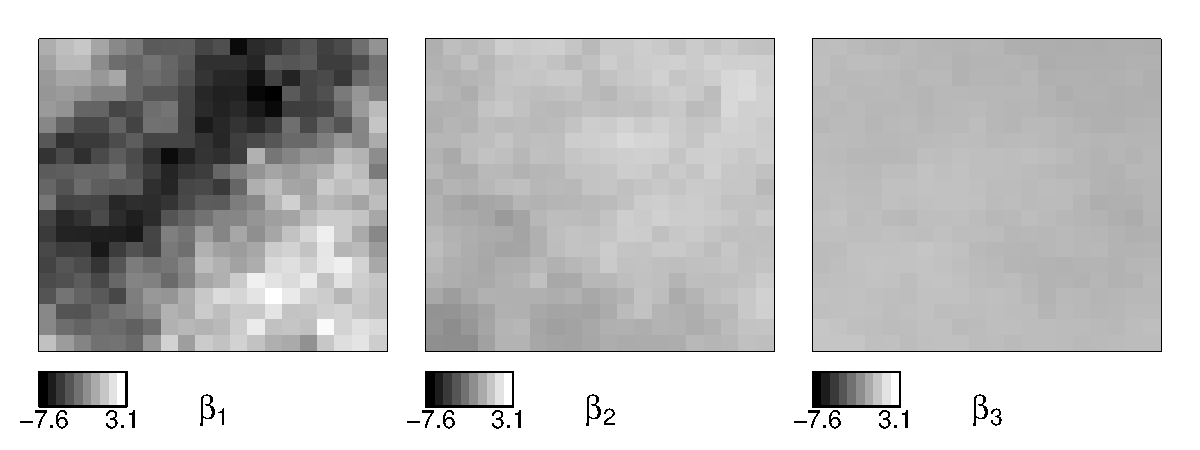
\includegraphics[width=\textwidth]{figure/coefs.pdf}
    \caption{Left to right, the values used for coefficients $\beta_1(\bm{s}), \dots, \beta_4(\bm{s})$ in the simulation study. \label{fig:simulation-coefficients}}
\end{figure}

Two parameters were varied to produce six simulation settings.
Data were simulated with low ($\rho=0$), medium ($\rho=0.5$), or high ($\rho=0.9$)
correlation between the covariates, and with
low ($\sigma_{\varepsilon}=0.5$) or high ($\sigma_{\varepsilon}=1$)
variance for the random error term. Each setting was used to generate one data set consisting of 400 observations.
For each data set, three estimates were made of the coefficients under three different sample sizes $n$: the full 400 observations, and subsets generated by sampling 100 or 200 unique observations uniformly from the data set.
The coefficients were estimated via LAGR and via a VCR model without variable selection as in Section \ref{sec:lagr-gaussian}.
For both estimation methods, the bandwidth parameter was $h=(1/2)n^{-1/6}$.

The results are presented in terms of the mean integrated squared
error (MISE) of the coefficient surface estimates $\hat{\beta}_{1}(\bm{s}),\dots,\hat{\beta}_{5}(\bm{s})$,
the MISE of the fitted response $\hat{y}(\bm{s})$, and the frequency
with which the coefficient surface estimates $\hat{\beta}_{1}(\bm{s}),\dots,\hat{\beta}_{5}(\bm{s})$
estimated by LAGR were zero.

\begin{table}
	\centering
	\begin{tabular}{|ccc|cc|cc|cc|cc|}
		\hline
		\multicolumn{3}{|c|}{\begin{tabular}[c]{@{}c@{}}Simulation\\settings\end{tabular}} & \multicolumn{2}{c|}{\begin{tabular}[c]{@{}c@{}}MISE\\$\hat{\beta}_1$\end{tabular}} & \multicolumn{2}{c|}{\begin{tabular}[c]{@{}c@{}}MISE\\$\hat{\beta}_2$\end{tabular}} & \multicolumn{2}{c|}{\begin{tabular}[c]{@{}c@{}}MISE\\$\hat{\beta}_3$\end{tabular}} & \multicolumn{2}{c|}{\begin{tabular}[c]{@{}c@{}}MISE\\$\hat{\beta}_4$\end{tabular}} \\
		$n$ & $\rho$ & $\sigma_{\varepsilon}$ & LAGR & VCR & LAGR & VCR & LAGR & VCR & LAGR & VCR \\
		\hline 

% latex table generated in R 3.1.1 by xtable 1.7-4 package
% Wed Sep 17 17:52:23 2014
  \multirow{6}{*}{100} & \multirow{2}{*}{0} & 0.5 & \textbf{1.18} & 1.25 & \textbf{0.37} & 0.41 & \textbf{0.10} & 0.14 & \textbf{0.03} & 0.09 \\ 
    &  & 1.0 & \textbf{1.75} & 1.90 & \textbf{0.62} & 0.85 & \textbf{0.42} & 0.57 & \textbf{0.17} & 0.25 \\ 
    & \multirow{2}{*}{0.5} & 0.5 & \textbf{1.65} & 1.75 & \textbf{0.30} & 0.41 & \textbf{0.12} & 0.21 & \textbf{0.41} & 0.62 \\ 
    &  & 1.0 & \textbf{1.13} & 1.15 & 0.33 & \textbf{0.21} & \textbf{0.05} & 0.11 & \textbf{0.22} & 0.43 \\ 
    & \multirow{2}{*}{0.9} & 0.5 & \textbf{2.71} & 3.40 & \textbf{1.33} & 3.07 & \textbf{1.46} & 2.81 & \textbf{1.54} & 2.87 \\ 
    &  & 1.0 & \textbf{2.00} & 2.66 & \textbf{0.81} & 1.38 & \textbf{0.23} & 0.88 & \textbf{0.68} & 1.67 \\ 
   \hline \multirow{6}{*}{200} & \multirow{2}{*}{0} & 0.5 & \textbf{1.19} & 1.23 & \textbf{0.16} & 0.17 & \textbf{0.11} & 0.20 & \textbf{0.05} & 0.09 \\ 
    &  & 1.0 & \textbf{1.15} & 1.15 & 0.39 & \textbf{0.28} & \textbf{0.04} & 0.11 & \textbf{0.06} & 0.21 \\ 
    & \multirow{2}{*}{0.5} & 0.5 & \textbf{1.33} & 1.42 & 0.17 & \textbf{0.17} & \textbf{0.07} & 0.14 & \textbf{0.05} & 0.14 \\ 
    &  & 1.0 & \textbf{1.18} & 1.26 & 0.39 & \textbf{0.36} & \textbf{0.04} & 0.04 & \textbf{0.02} & 0.12 \\ 
    & \multirow{2}{*}{0.9} & 0.5 & \textbf{2.41} & 2.57 & \textbf{0.73} & 1.13 & \textbf{0.41} & 0.96 & \textbf{0.66} & 0.92 \\ 
    &  & 1.0 & \textbf{2.07} & 2.32 & \textbf{0.69} & 1.27 & \textbf{0.12} & 0.39 & \textbf{0.11} & 0.59 \\ 
   \hline \multirow{6}{*}{400} & \multirow{2}{*}{0} & 0.5 & \textbf{1.20} & 1.21 & 0.17 & \textbf{0.17} & \textbf{0.06} & 0.07 & \textbf{0.03} & 0.06 \\ 
    &  & 1.0 & 1.14 & \textbf{1.11} & 0.18 & \textbf{0.18} & \textbf{0.05} & 0.07 & \textbf{0.02} & 0.06 \\ 
    & \multirow{2}{*}{0.5} & 0.5 & 1.25 & \textbf{1.24} & \textbf{0.19} & 0.25 & \textbf{0.05} & 0.08 & \textbf{0.01} & 0.09 \\ 
    &  & 1.0 & 1.20 & \textbf{1.19} & 0.32 & \textbf{0.29} & \textbf{0.05} & 0.08 & \textbf{0.03} & 0.07 \\ 
    & \multirow{2}{*}{0.9} & 0.5 & \textbf{1.50} & 1.60 & \textbf{0.39} & 0.39 & \textbf{0.35} & 0.54 & \textbf{0.42} & 0.63 \\ 
    &  & 1.0 & \textbf{1.38} & 1.72 & \textbf{0.44} & 0.68 & \textbf{0.14} & 0.33 & \textbf{0.03} & 0.25 \\ 

  
	\hline
	\end{tabular}
	\caption{For each setting as a combination of sample size $n$, cross-covariate correlation $\rho$, and error standard deviation $\sigma_{\varepsilon}$, the mean integrated squared error (MISE) of the coefficient estimates. The MISE of $\hat{\beta}_1, \dots, \hat{\beta}_5$ from estimation by local adaptive grouped regularization (LAGR) is compared to that from estimation by locally linear regression without selection (VCR). Highlighting indicates the \textbf{smallest} MISE for $\hat{\beta}_1, \dots, \hat{\beta}_5$.}
	\label{tab:mise}
\end{table}


\subsection{Simulation Results}

The MISE of the coefficient surface estimates are in Table \ref{tab:mise}.
For all coefficients, the MISE was more often lower under estimation by LAGR than under estimation by VCR.
The frequency with which MISE was lower under LAGR than under VCR for estimating $\beta_1$ was $12$ of $18$ cases, and was higher for all other covariates.
The improvement by MISE of LAGR over VCR was greater for covariates with smaller influence, with LAGR producing the smaller MISE for 



The MISE of true nonzero coefficient $\hat{\beta}_{1}(\bm{s})$ was
always the smallest under oracular selection. The difference in MISE
of $\hat{\beta}_{1}(\bm{s})$ under LAGR versus VCR estimation was
small and each method produced the smaller MISE for nine of $18$
settings. For both LAGR and VCR estimation, the MISE of $\hat{\beta}_{1}(\bm{s})$ under the settings with high cross-covariate correlation ($\rho=0.9$) and high noise variance ($\sigma_{\varepsilon}=1$) was about three times greater than under any of the other settings. 
Under these settings, coefficient estimation is difficult because the signal is buried in noise and what signal can be discerned is difficult to attribute to a specific covariate because all five are highly correlated. In the absence of either complication, coefficient estimation would be more accurate, as seen by the other entries in Table \ref{tab:mise} and by the fact that oracular selection (which eliminates any cross-covariate correlation in this simulation) did not experience a jump in MISE of $\hat{\beta}_{1}(\bm{s})$ under any simulation settings.

Recall that $\beta_{2}(\bm{s}),\dots,\beta_{5}(\bm{s})$
are exactly zero across the entire domain. Oracle selection will estimate
these coefficients perfectly, so we focus on the comparison between
estimation by LAGR and by the VCR model with no selection. These results
show that for every simulation setting, LAGR estimation of $\beta_{2}(\bm{s}),\dots,\beta_{5}(\bm{s})$
is more accurate than the standard VCR model. In particular, the MISE of $\beta_{2}(\bm{s}),\dots,\beta_{5}(\bm{s})$ for settings combining high cross-covariate correlation and high noise variance is at least five times higher under VCR estimation than under LAGR estimation.

From Table \ref{tab:misey}
we see that LAGR has good ability to identify zero-coefficient covariates.
The frequency with which $\beta_{2}(\bm{s}),\dots,\beta_{5}(\bm{s})$
were dropped from the LAGR models ranged from 0.78
to 0.97. The MISE of the fitted response $\hat{y}(\bm{s})$
is listed in Table \ref{tab:misey}, where the highlighting is based
on which methods estimate an error variance that is closest to the
known truth for the simulation. The results are all very similar to
each other, indicating that no method was consistently better than
the others in this simulation at fitting the response.

\begin{table}
	\centering
	\begin{tabular}{|ccc|cccc|cc|}
		\hline
		\multicolumn{3}{|c|}{\begin{tabular}[c]{@{}c@{}}Simulation\\settings\end{tabular}} &  \multicolumn{4}{c|}{\begin{tabular}[c]{@{}c@{}}Zero\\frequency\end{tabular}} &  \multicolumn{2}{c|}{\begin{tabular}[c]{@{}c@{}}MISE\\$\hat{y}$\end{tabular}} \\
		$n$ & $\rho$ & $\sigma_{\varepsilon}$ & $\hat{\beta}_1$ & $\hat{\beta}_2$ & $\hat{\beta}_3$ & $\hat{\beta}_4$ & LAGR & VCR \\
		\hline 

% latex table generated in R 3.1.1 by xtable 1.7-4 package
% Wed Sep 17 17:52:23 2014
  \multirow{6}{*}{100} & \multirow{2}{*}{0} & 0.5 & 0.00 & 0.22 & 0.43 & 0.85 & 1.00 & \textbf{0.81} \\ 
    &  & 1.0 & 0.00 & 0.12 & 0.23 & 0.30 & 1.43 & \textbf{1.31} \\ 
    & \multirow{2}{*}{0.5} & 0.5 & 0.00 & 0.18 & 0.57 & 0.10 & 1.04 & \textbf{0.87} \\ 
    &  & 1.0 & 0.00 & 0.48 & 0.93 & 0.54 & 1.65 & \textbf{1.17} \\ 
    & \multirow{2}{*}{0.9} & 0.5 & 0.43 & 0.47 & 0.52 & 0.22 & 1.16 & \textbf{0.89} \\ 
    &  & 1.0 & 0.10 & 0.68 & 0.52 & 0.48 & 1.25 & \textbf{1.00} \\ 
   \hline \multirow{6}{*}{200} & \multirow{2}{*}{0} & 0.5 & 0.00 & 0.10 & 0.40 & 0.56 & 1.16 & \textbf{1.10} \\ 
    &  & 1.0 & 0.00 & 0.76 & 0.89 & 0.74 & 2.38 & \textbf{2.04} \\ 
    & \multirow{2}{*}{0.5} & 0.5 & 0.00 & 0.32 & 0.64 & 0.62 & 1.35 & \textbf{1.19} \\ 
    &  & 1.0 & 0.00 & 0.62 & 0.95 & 0.86 & 1.57 & \textbf{1.41} \\ 
    & \multirow{2}{*}{0.9} & 0.5 & 0.14 & 0.34 & 0.50 & 0.28 & 1.37 & \textbf{1.20} \\ 
    &  & 1.0 & 0.05 & 0.10 & 0.66 & 0.74 & 1.84 & \textbf{1.64} \\ 
   \hline \multirow{6}{*}{400} & \multirow{2}{*}{0} & 0.5 & 0.00 & 0.06 & 0.38 & 0.53 & 1.19 & \textbf{1.15} \\ 
    &  & 1.0 & 0.00 & 0.21 & 0.47 & 0.64 & 2.16 & \textbf{2.00} \\ 
    & \multirow{2}{*}{0.5} & 0.5 & 0.00 & 0.16 & 0.76 & 0.79 & 1.75 & \textbf{1.56} \\ 
    &  & 1.0 & 0.00 & 0.29 & 0.70 & 0.78 & 1.68 & \textbf{1.58} \\ 
    & \multirow{2}{*}{0.9} & 0.5 & 0.00 & 0.43 & 0.47 & 0.31 & 1.56 & \textbf{1.39} \\ 
    &  & 1.0 & 0.00 & 0.26 & 0.73 & 0.80 & 2.38 & \textbf{2.20} \\ 


  
	\hline
	\end{tabular}
	\caption{For each setting as a combination of sample size $n$, cross-covariate correlation $\rho$, and error standard deviation $\sigma_{\varepsilon}$, the frequency of exact zeroes in the estimates of $\hat{\beta}_2,\dots,\hat{\beta}_5$ as estimated by local adaptive grouped regularizaton (LAGR). Also, the mean integrated squared error (MISE) for the fitted output of each simulation setting, under variable selection via LAGR, locally linear regression without selection (VCR), and by locally linear regression with oracular selection (Oracle). Highlighting indicates the \textbf{closest} and \emph{next-closest} to the actual error variance $\sigma_\varepsilon^2$ for that simulation setting.}
	\label{tab:misey}
\end{table}

Overall, the proposed LAGR method was accurate in variable selection
and coefficient surface estimation, with estimation accuracy for $\beta_{1}(\bm{s})$
about equal to that of the VCR model with no selection, and with consistently
better accuracy for estimating $\beta_{2}(\bm{s}),\dots,\beta_{5}(\bm{s})$.
There was little difference in the performance of the proposed LAGR
method between low ($\sigma_{\varepsilon}=0.5$) and high ($\sigma_{\varepsilon}=1$)
error variance, and between no ($\rho=0$) and moderate ($\rho=0.5$)
correlation among the covariates. But the selection and estimation
accuracy did decline when there was high ($\rho=0.9$) correlation
among the covariates.


\section{Data Example\label{sec:example}}




The proposed LAGR estimation method was applied to estimate the coefficients
in a VCR model of the effect of some covariates on the price of homes
in Boston based on data from the 1970 U.S. census \citep{Harrison-Rubinfeld-1978,Gilley-Pace-1996,Pace-Gilley-1997}.
The data are the median price of homes sold in 506 census tracts (MEDV),
along with the potential covariates CRIM (the per-capita crime rate
in the tract), RM (the mean number of rooms for houses sold in the
tract), RAD (an index of how accessible the tract is from Boston's
radial roads), TAX (the property tax per \$10,000 of property value),
and LSTAT (the percentage of the tract's residents who are considered
``lower status''). With the Epanechnikov kernel, the bandwidth parameter
was set to 0.2 for a nearest neighbors-type bandwidth, meaning that
the sum of kernel weights for each local model was 20\% of the total
number of observations.

A summary of the estimates of the local coefficients is in Table \ref{tab:boston-coefs-lagr}.
It indicates that RM is the only covariate with a positive mean local
coefficient estimate. The percentage of census tracts where the local
coefficient was estimated to be exactly zero was 1\%
for LSTAT, 2\%
for RM, 37\%
for RAD, 49\%
for CRIM, and 100\%
for TAX.

\begin{figure}

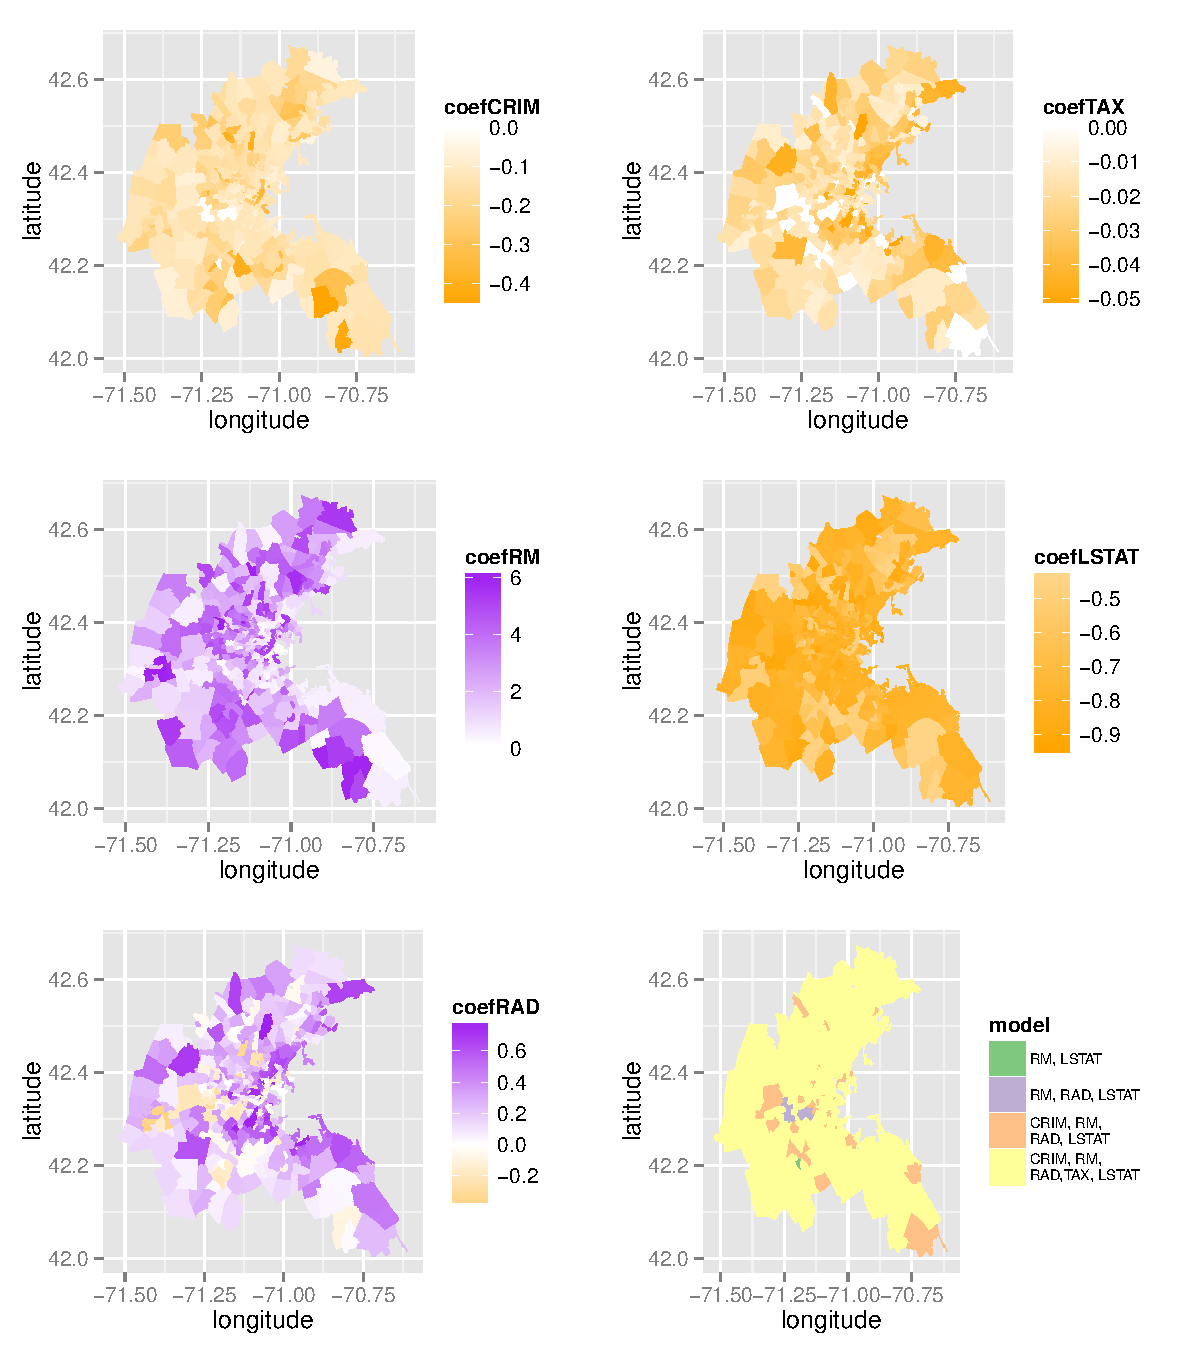
\includegraphics[width=\maxwidth]{figure/boston-plots} 


\caption{Coefficients for the Boston house price data as estimated by local adaptive grouped regularization.\label{fig:boston-lagr-coefs}}
\end{figure}

The estimates of the local coefficients are plotted in Figure \ref{fig:boston-lagr-coefs}.
One interesting result is that the TAX variable was nowhere found
to be associated with of the median house price. Another is that the
coefficients of CRIM and LSTAT are everywhere negative or zero (meaning
that a greater crime rate or proportion of lower-status individuals
is associated with a lower median house price where the effect is
discernible) and that of RM is positive (meaning that a greater average
number of rooms per house is associated with a greater median house
price). The coefficient of RAD is positive in some areas and negative
in others. This indicates that there are parts of Boston where access
to radial roads is associated with a greater median house price and
parts where it is associated with a lesser median house price.

% latex table generated in R 3.1.1 by xtable 1.7-3 package
% Mon Aug 18 22:12:11 2014
\begin{table}
\centering
\begin{tabular}{|c|ccc|}
  \hline
 & Mean & SD & Prop. zero \\ 
  \hline
CRIM & -0.07 & 0.08 & 0.49 \\ 
  RM & 1.92 & 1.43 & 0.02 \\ 
  RAD & -0.08 & 0.13 & 0.37 \\ 
  TAX & 0.00 & 0.00 & 1.00 \\ 
  LSTAT & -0.72 & 0.16 & 0.01 \\ 
   \hline
\end{tabular}
\caption{The mean, standard deviation, and proportion of zeros among the estimates of the local coefficients in a model for the median house price in census tracts in Boston, with coefficients selected and fitted by local adaptive grouped regularization. The covariates are CRIM (per capita crime rate in the census tract), RM (average number of rooms per home sold in the census tract), RAD (an index of the tract's access to radial roads), TAX (property tax per USD10,000 of property value), and LSTAT (percentage of the tract's residents who are considered ``lower status").} 
\label{tab:boston-coefs-lagr}
\end{table}


In their example using the same data, \citet{Sun-Yan-Zhang-Lu-2014}
estimated that the coefficients of RAD and LSTAT should be constant,
at $0.36$ and $-0.45$, respectively. That conclusion differs from
our result, which says that the mean estimated local coefficient of
RAD is actually negative (\ensuremath{-0.08}),
while our mean fitted local coefficient for LSTAT was more negative
than the estimate of \citet{Sun-Yan-Zhang-Lu-2014}.


\section{Extension to Generalized Linear Regression\label{sec:lagr-gllm}}


\subsection{Local GLM and Local Quasi-likelihood Estimation}

Generalized linear models (GLMs) extend the linear regression model
to a response variable following any distribution in the exponential
family \citep{McCullagh-Nelder-1989}. As is the case for the local
linear regression model, we now consider local GLM coefficients as
smooth functions of location \citep{Cai-Fan-Li-2000}. Suppose the
response variable $Y$ is from an exponential family distribution
with $E\left\{ y(\bm{s})|\bm{x}(\bm{s})\right\} =\mu(\bm{s})=b'\left(\theta(\bm{s})\right)$,
$\theta(\bm{s})=(g\circ b')^{-1}\left(\eta(\bm{s})\right)$, $\eta(\bm{s})=\bm{x}(\bm{s})^{T}\bm{\beta}(\bm{s})=g\left(\mu(\bm{s})\right)$,
$\text{\text{Var}}\left\{ y(\bm{s})|\bm{x}(\bm{s})\right\} =b''\left(\theta(\bm{s})\right)$,
and link function $g(\cdot)$. Then the probability density is 

\[
f\left(y(\bm{s})|\bm{x}(\bm{s}),\theta(\bm{s})\right)=c\left(y(\bm{s})\right)\times\exp\left\{ \theta(\bm{s})y(\bm{s})-b\left(\theta(\bm{s})\right)\right\} .
\]


If $g^{-1}(\cdot)=b'(\cdot)$, then the composition $(g\circ b')(\cdot)$
is the identity function. This particular $g$ is called the canonical
link. Assuming the canonical link, all that is required is to specify
the mean-variance relationship via the variance function, $V\left(\mu(\bm{s})\right)$.
Then the local coefficients can be estimated by maximizing the local
quasi-likelihood 

\begin{align}
\mathcal{\ell}^{*}\left(\bm{\zeta}(\bm{s})\right) & =\sum_{i=1}^{n}K_{h}\left(\|\bm{s}-\bm{s}_{i}\|\right)Q\left(g^{-1}\left(\bm{z}_{i}^{T}\bm{\zeta}(\bm{s})\right),Y_{i}\right).\label{eq:local-quasi-likelihood}
\end{align}


The local quasi-likelihood (\ref{eq:local-quasi-likelihood}) generalizes
the local log-likelihood (\ref{eq:local-log-likelihood}) that was
used to estimate coefficients in the local linear regression. The
local quasi-likelihood (\ref{eq:local-quasi-likelihood}) is convex,
and is defined in terms of its derivative, the local quasi-score function
$\left(\partial/\partial\mu\right)Q(\mu,y)=(y-\mu)\{V(\mu)\}^{-1}$.
The local quasi-likelihood is maximized by setting the local quasi-score
function to zero:

\begin{align}
(\partial/\partial\bm{\zeta})\mathcal{\ell}^{*}\left(\hat{\bm{\zeta}}(\bm{s})\right) & =\sum_{i=1}^{n}K_{h}\left(\|\bm{s}-\bm{s}_{i}\|\right)\left(y_{i}-\hat{\mu}(\bm{s}_{i};\bm{s})\right)\left\{ V\left(\hat{\mu}(\bm{s}_{i};\bm{s})\right)\right\} ^{-1}\bm{z}_{i}=\bm{0}_{3p},
\end{align}


where $\hat{\mu}(\bm{s}_{i};\bm{s})=g^{-1}\left(\bm{z}_{i}^{T}\hat{\bm{\zeta}}(\bm{s})\right)$
is the mean at location $\bm{s}_{i}$ evaluated at the estimated coefficients
$\hat{\bm{\zeta}}(\bm{s})$ at location $\bm{s}$. The asymptotic
distribution of the local coefficients in a varying-coefficient GLM
with a one-dimensional effect-modifying parameter are given in \citet{Cai-Fan-Li-2000}.
For coefficients that vary in the two dimensions, the arguments in
the proof of Theorem 1 of \citet{Cai-Fan-Li-2000} can be extended
to show that the distribution of the estimated local coefficients
is:

\begin{gather*}
\left\{ nh^{2}f(\bm{s})\right\} ^{1/2}\left[\tilde{\bm{\beta}}(\bm{s})-\bm{\beta}(\bm{s})-(1/2)\kappa_{0}^{-1}\kappa_{2}h^{2}\left\{ \nabla_{uu}^{2}\bm{\beta}(\bm{s})+\nabla_{vv}^{2}\bm{\beta}(\bm{s})\right\} \right]\\
\xrightarrow{{D}}N\left(\bm{0},\kappa_{0}^{-2}\nu_{0}\bm{\Gamma}(\bm{s})^{-1}\right).
\end{gather*}



\subsection{LAGR Penalized Local Likelihood and Oracle Properties}

Whereas the method of LAGR for local linear regression uses a penalized
local likelihood, LAGR for GLMs uses a penalized local quasi-likelihood:

\begin{align*}
\mathcal{J}\left(\bm{\zeta}(\bm{s})\right)= & \mathcal{\ell}^{*}\left(\bm{\zeta}(\bm{s})\right)+\mathcal{P}\left(\bm{\zeta}(\bm{s})\right)\\
= & \sum_{i=1}^{n}K_{h}\left(\|\bm{s}-\bm{s}_{i}\|\right)Q\left(g^{-1}\left(\bm{z}_{i}^{T}\bm{\zeta}(\bm{s})\right),Y_{i}\right)+\sum_{j=1}^{p}\phi_{j}(\bm{s})\|\bm{\zeta}_{(j)}(\bm{s})\|.
\end{align*}


Further, let $\phi_{j}(\bm{s})=\lambda_{n}\|\tilde{\bm{\zeta}}_{(j)}(\bm{s})\|^{-\gamma}$,
where $\lambda_{n}>0$ is a the local tuning parameter applied to
all coefficients at location $\bm{s}$ and $\tilde{\bm{\zeta}}_{(j)}(\bm{s})$
is the vector of unpenalized local coefficients. The following are
additional to the definitions and conditions of Section \ref{sub:oracle-properties}.
Define $\rho(\bm{s},\bm{z})=\left[g_{1}\left(\mu(\bm{s},\bm{z})\right)\right]^{2}Var\left\{ Y(\bm{s})|\bm{X}(\bm{s}),\bm{s}\right\} $,
where $g_{1}(\cdot)=g'_{0}(\cdot)/g'(\cdot)$, and $g_{0}(\cdot)$
is the canonical link function. So when the canonical link is used,
$\rho(\bm{s},\bm{z})=V\left(\mu(\bm{s},\bm{z})\right)$. Let $\bm{\Gamma}\left(\bm{s}\right)=E\left\{ \rho\left(\bm{s},\bm{X}(\bm{s})\right)\bm{X}(\bm{s})\bm{X}(\bm{s})^{T}|\bm{s},\bm{Z}(\bm{s})=\bm{z}\right\} $
and 
\[
\bm{\Gamma}_{(a)}\left(\bm{s}\right)=E\left\{ \rho\left(\bm{s},\bm{X}_{(a)}(\bm{s})\right)\bm{X}_{(a)}(\bm{s})\bm{X}_{(a)}(\bm{s})^{T}|\bm{s},\bm{Z}(\bm{s})=\bm{z}\right\} .
\]
Assume the following regularity conditions:
\begin{itemize}
\item[(C.8)] The functions $g'''\left(\bm{s}\right)$, $\nabla\bm{\Gamma}\left(\bm{s}\right)$,
$\nabla\bm{\Gamma}_{(a)}\left(\bm{s}\right)$, $V\left(\mu\left(\bm{s},\bm{z}\right)\right)$,
and $V'\left(\mu\left(\bm{s},\bm{z}\right)\right)$ are continuous
at $\bm{s}$.
\item[(C.9)] The function $\left(\partial^{2}/\partial\mu^{2}\right)Q\left(g^{-1}\left(\mu\right),y\right)<0$
for $\mu\in\mathbb{R}$ and $y$ in the range of the response.
\end{itemize}
These additional conditions are not uncommon in the nonparametric
regression literature (see, e.g., conditions (1) and (2) of \citet{Cai-Fan-Li-2000}).
Condition (C.8) is needed for the Taylor's expansion of the local
quasi-likelihood. Condition (C.9) assures that the local quasi-likelihood
is convex and has a unique minimizer.
\begin{thm}[Asymptotic normality]
\label{theorem:normality-glm}  Under (C.1)--(C.10),
\begin{gather*}
\left\{ nh^{2}f(\bm{s})\right\} ^{1/2}\left[\hat{\bm{\beta}}_{(a)}(\bm{s})-\bm{\beta}_{(a)}(\bm{s})-\left(2\kappa_{0}\right)^{-1}\kappa_{2}h^{2}\left\{ \nabla_{uu}^{2}\bm{\beta}_{\left(a\right)}(\bm{s})+\nabla_{vv}^{2}\bm{\beta}_{\left(a\right)}(\bm{s})\right\} \right]\\
\xrightarrow{d}N\left(0,\kappa_{0}^{-2}\nu_{0}\bm{\Gamma}_{(a)}(\bm{s})^{-1}\right)
\end{gather*}
\end{thm}

\begin{thm}[Selection consistency]
\label{theorem:selection-glm}  Under (C.1)--(C.10),
\[
P\left\{ \|\hat{\bm{\zeta}}_{(j)}(\bm{s})\|=\bm{0}\right\} \to1\text{ if }j>p_{0}.
\]
 
\end{thm}
By Theorem \ref{theorem:normality-glm}, the LAGR estimates achieve
the same asymptotic distribution as if the nonzero coefficients were
known in advance. The difference between the Gaussian and GLM cases
is that $\sigma^{2}\bm{\Psi}_{(a)}(\bm{s})^{-1}$ in the variance
term of Theorem \ref{theorem:normality} has been replaced by $\bm{\Gamma}_{(a)}(\bm{s})^{-1}$
in Theorem \ref{theorem:normality-glm} because the variance of the
response in the GLM case depends on the expectation of the response.
Theorem \ref{theorem:selection-glm} gives the same result for the
GLM setting as Theorem \ref{theorem:selection} does for the Gaussian
setting: the true zero coefficients are dropped from the model with
probability tending to one. Thus, the oracle properties for the GLM
setting are established. The technical proofs are given in Appendix
B and the necessary lemmas are provided in the online supplementary
materials.


\section{Conclusions and Discussion}

We have developed a new method of LAGR and shown its oracle properties
for local variable selection and coefficient estimation in VCR models.
This is in contrast to the existing literature on variable selection
for VCR models that focuses on global variable selection. Further,
the method of LAGR extends the adaptive group lasso. In particular,
the previous literature on the adaptive group lasso is insufficient
for local selection in a VCR model because the local weights are functions
of the kernel $K(\cdot)$ and the bandwidth $h$. As a result, the
local observation weights change with sample size and the coefficient
estimates converge at a slower rate than in the traditional adaptive
group lasso. Thus, the conditions for oracle properties of the adaptive
group lasso must be refined for the LAGR method.

Here we considered the case of two-dimensional effect-modifying parameter.
Similar results can be obtained when the effect-modifying parameter
has dimension other than two, but in higher dimensions the so-called
``curse of dimensionality'' means that the estimation accuracy quickly
degrades. Since the optimal rate of convergence for nonparametric
regression is achieved when $h=O\left(n^{-1/\{4+d\}}\right)$ where
$d$ is the dimension of the effect-modifying parameter, it follows
that to attain the oracle properties, the exponent in the adaptive
weights for LAGR estimation must satisfy $\gamma>d/2$.


\section*{References}
\bibliographystyle{chicago}
\begin{thebibliography}{}

\bibitem[\protect\citeauthoryear{Akaike}{Akaike}{1973}]{Akaike-1973}
Akaike, H. (1973).
\newblock Information theory and an extension of the maximum likelihood
  principle.
\newblock In B.~Petrov and F.~Csaki (Eds.), {\em 2nd International Symposium on
  Information Theory}, pp.\  267--281.

\bibitem[\protect\citeauthoryear{Antoniadas, Gijbels, and
  Verhasselt}{Antoniadas et~al.}{2012}]{Antoniadis:2012a}
Antoniadas, A., I.~Gijbels, and A.~Verhasselt (2012).
\newblock Variable selection in varying-coefficient models using {P}-splines.
\newblock {\em Journal of Computational and Graphical Statistics\/}~{\em 21},
  638--661.

\bibitem[\protect\citeauthoryear{Cai, Fan, and Li}{Cai
  et~al.}{2000}]{Cai-Fan-Li-2000}
Cai, Z., J.~Fan, and R.~Li (2000).
\newblock Efficient estimation and inferences for varying-coefficient models.
\newblock {\em Journal of the American Statistical Association\/}~{\em 95},
  888--902.

\bibitem[\protect\citeauthoryear{Cleveland and Grosse}{Cleveland and
  Grosse}{1991}]{Cleveland-Grosse-1991}
Cleveland, W. and E.~Grosse (1991).
\newblock Local regression models.
\newblock In J.~Chambers and T.~Hastie (Eds.), {\em Statistical models in S}.
  Wadsworth and Brooks/Cole.

\bibitem[\protect\citeauthoryear{Efron}{Efron}{2004}]{Efron:2004a}
Efron, B. (2004).
\newblock The estimation of prediction error: covariance penalties and
  cross-validation.
\newblock {\em Journal of the American Statistical Association\/}~{\em 99},
  619--632.

\bibitem[\protect\citeauthoryear{Fan and Gijbels}{Fan and
  Gijbels}{1996}]{Fan-Gijbels-1996}
Fan, J. and I.~Gijbels (1996).
\newblock {\em Local Polynomial Modeling and its Applications}.
\newblock Chapman and Hall, London.

\bibitem[\protect\citeauthoryear{Fan and Zhang}{Fan and
  Zhang}{1999}]{Fan-Zhang-1999}
Fan, J. and W.~Zhang (1999).
\newblock Statistical estimation in varying coefficient models.
\newblock {\em Annals of Statistics\/}~{\em 27}, 1491--1518.

\bibitem[\protect\citeauthoryear{Geyer}{Geyer}{1994}]{Geyer-1994}
Geyer, C.~J. (1994).
\newblock On the asymptotics of constrained ${M}$-estimation.
\newblock {\em Annals of Statistics\/}~{\em 22}, 1993--2010.

\bibitem[\protect\citeauthoryear{Gilley and Pace}{Gilley and
  Pace}{1996}]{Gilley-Pace-1996}
Gilley, O. and R.~K. Pace (1996).
\newblock On the {H}arrison and {R}ubinfeld data.
\newblock {\em Journal of Environmental Economics and Management\/}~{\em 31},
  403--405.

\bibitem[\protect\citeauthoryear{Harrison and Rubinfeld}{Harrison and
  Rubinfeld}{1978}]{Harrison-Rubinfeld-1978}
Harrison, D. and D.~L. Rubinfeld (1978).
\newblock Hedonic housing prices and the demand for clean air.
\newblock {\em Journal of Environmental Economics and Management\/}~{\em 5},
  81--102.

\bibitem[\protect\citeauthoryear{Hastie and Loader}{Hastie and
  Loader}{1993}]{Hastie:1993b}
Hastie, T. and C.~Loader (1993).
\newblock Local regression: automatic kernel carpentry.
\newblock {\em Statistical Science\/}~{\em 8}, 120--143.

\bibitem[\protect\citeauthoryear{Hastie and Tibshirani}{Hastie and
  Tibshirani}{1993}]{Hastie-Tibshirani-1993}
Hastie, T. and R.~Tibshirani (1993).
\newblock Varying-coefficient models.
\newblock {\em Journal of the Royal Statistical Society Series B\/}~{\em 55},
  757--796.

\bibitem[\protect\citeauthoryear{Hurvich, Simonoff, and Tsai}{Hurvich
  et~al.}{1998}]{Hurvich-1998}
Hurvich, C.~M., J.~S. Simonoff, and C.-L. Tsai (1998).
\newblock Smoothing parameter selection in nonparametric regression using an
  improved {A}kaike information criterion.
\newblock {\em Journal of the Royal Statistical Society Series B\/}~{\em 60},
  271--293.

\bibitem[\protect\citeauthoryear{Knight and Fu}{Knight and
  Fu}{2000}]{Knight-Fu-2000}
Knight, K. and W.~Fu (2000).
\newblock Asymptotics for {L}asso-type estimators.
\newblock {\em Annals of Statistics\/}~{\em 28}, 1356--1378.

\bibitem[\protect\citeauthoryear{Mallows}{Mallows}{1973}]{Mallows-1973}
Mallows, C. (1973).
\newblock Some comments on ${C}_p$.
\newblock {\em Technometrics\/}~{\em 15}, 661--675.

\bibitem[\protect\citeauthoryear{McCullagh and Nelder}{McCullagh and
  Nelder}{1989}]{McCullagh-Nelder-1989}
McCullagh, P. and J.~Nelder (1989).
\newblock {\em Generalized Linear Models, Second Edition}.
\newblock Taylor and Francis.

\bibitem[\protect\citeauthoryear{Pace and Gilley}{Pace and
  Gilley}{1997}]{Pace-Gilley-1997}
Pace, R.~K. and O.~Gilley (1997).
\newblock Using the spatial configuration of the data to improve estimation.
\newblock {\em Journal of Real Estate Finance and Economics\/}~{\em 14},
  333--340.

\bibitem[\protect\citeauthoryear{Samiuddin and el~Sayyad}{Samiuddin and
  el~Sayyad}{1990}]{Samiuddin-el-Sayyad-1990}
Samiuddin, M. and G.~M. el~Sayyad (1990).
\newblock On nonparametric kernel density estimates.
\newblock {\em Biometrika\/}~{\em 77}, 865--874.

\bibitem[\protect\citeauthoryear{Stein}{Stein}{1981}]{Stein-1981}
Stein, C. (1981).
\newblock Estimation of the mean of a multivariate normal distribution.
\newblock {\em Annals of Statistics\/}~{\em 9}, 1135--1151.

\bibitem[\protect\citeauthoryear{Sun, Yan, Zhang, and Lu}{Sun
  et~al.}{2014}]{Sun-Yan-Zhang-Lu-2014}
Sun, Y., H.~Yan, W.~Zhang, and Z.~Lu (2014).
\newblock A semiparametric spatial dynamic model.
\newblock {\em Annals of Statistics\/}~{\em 42}, 700--727.

\bibitem[\protect\citeauthoryear{Tibshirani}{Tibshirani}{1996}]{Tibshirani-1996}
Tibshirani, R. (1996).
\newblock Regression shrinkage and selection via the {L}asso.
\newblock {\em Journal of the Royal Statistical Society Series B\/}~{\em 58},
  267--288.

\bibitem[\protect\citeauthoryear{Wang and Leng}{Wang and
  Leng}{2008}]{Wang-Leng-2008}
Wang, H. and C.~Leng (2008).
\newblock A note on adaptive group {L}asso.
\newblock {\em Computational Statistics and Data Analysis\/}~{\em 52},
  5277--5286.

\bibitem[\protect\citeauthoryear{Wang and Xia}{Wang and
  Xia}{2009}]{Wang-Xia-2009}
Wang, H. and Y.~Xia (2009).
\newblock Shrinkage estimation of the varying coefficient model.
\newblock {\em Journal of the American Statistical Association\/}~{\em 104},
  747--757.

\bibitem[\protect\citeauthoryear{Wang, Li, and Huang}{Wang
  et~al.}{2008}]{Wang-2008a}
Wang, L., H.~Li, and J.~Z. Huang (2008).
\newblock Variable selection in nonparametric varying-coefficient models for
  analysis of repeated measurements.
\newblock {\em Journal of the American Statistical Association\/}~{\em 103},
  1556--1569.

\bibitem[\protect\citeauthoryear{Wang, Mei, and Yan}{Wang
  et~al.}{2008}]{Wang-2008b}
Wang, N., C.-L. Mei, and X.-D. Yan (2008).
\newblock Local linear estimation of spatially varying coefficient models: an
  improvement on the geographically weighted regression technique.
\newblock {\em Environment and Planning A\/}~{\em 40}, 986--1005.

\bibitem[\protect\citeauthoryear{Yuan and Lin}{Yuan and
  Lin}{2006}]{Yuan-Lin-2006}
Yuan, M. and Y.~Lin (2006).
\newblock Model selection and estimation in regression with grouped variables.
\newblock {\em Journal of the Royal Statistical Society Series B\/}~{\em 68},
  49--67.

\bibitem[\protect\citeauthoryear{Zou}{Zou}{2006}]{Zou-2006}
Zou, H. (2006).
\newblock The adaptive {L}asso and its oracle properties.
\newblock {\em Journal of the American Statistical Association\/}~{\em 101},
  1418--1429.

\end{thebibliography}

\clearpage

\appendix
\section{Proofs of Theorems 1--2}
\subsection*{Proof of Theorem \ref{theorem:normality}\label{sec:gaussian-normality-proof} }
\begin{proof}
Let $H_{n}(\bm{u})=\mathcal{J}\left(\bm{\zeta}(\bm{s})+h^{-1}n^{-1/2}\bm{u}\right)-\mathcal{J}\left(\bm{\zeta}(\bm{s})\right)$
and $\alpha_{n}=h^{-1}n^{-1/2}$. Then, we have 
\begin{align*}
H_{n}(\bm{u})= & (1/2)\left[\bm{Y}-\bm{Z}(\bm{s})\left\{ \bm{\zeta}(\bm{s})+\alpha_{n}\bm{u}\right\} \right]^{T}\bm{W}\!(\bm{s})\left[\bm{Y}-\bm{Z}(\bm{s})\left\{ \bm{\zeta}(\bm{s})+\alpha_{n}\bm{u}\right\} \right]\\
 & +\sum_{j=1}^{p}\phi_{j}(\bm{s})\|\bm{\zeta}_{j}(\bm{s})+\alpha_{n}\bm{u}_{j}\|\\
 & -(1/2)\left\{ \bm{Y}-\bm{Z}(\bm{s})\bm{\zeta}(\bm{s})\right\} ^{T}\bm{W}\!(\bm{s})\left\{ \bm{Y}-\bm{Z}(\bm{s})\bm{\zeta}(\bm{s})\right\} -\sum_{j=1}^{p}\phi_{j}(\bm{s})\|\bm{\zeta}_{j}(\bm{s})\|\\
= & \left(1/2\right)\alpha_{n}^{2}\bm{u}^{T}\left\{ \bm{Z}(\bm{s})^{T}\bm{W}\!(\bm{s})\bm{Z}(\bm{s})\right\} \bm{u}\\
 & -\alpha_{n}\bm{u}^{T}\left[\bm{Z}(\bm{s})^{T}\bm{W}\!(\bm{s})\left\{ \bm{Y}-\bm{Z}(\bm{s})\bm{\zeta}(\bm{s})\right\} \right]\\
 & +\sum_{j=1}^{p}n^{-1/2}\phi_{j}(\bm{s})n^{1/2}\left\{ \|\bm{\zeta}_{(j)}(\bm{s})+\alpha_{n}\bm{u}_{(j)}\|-\|\bm{\zeta}_{(j)}(\bm{s})\|\right\} .
\end{align*}
The limiting behavior of the last term differs between the cases $j\le p_{0}$
and $j>p_{0}$.
\emph{Case $j\le p_{0}$}: If $j\le p_{0}$, then $n^{-1/2}\phi_{j}(\bm{s})\to n^{-1/2}\lambda_{n}\|\bm{\zeta}_{(j)}(\bm{s})\|^{-\gamma}$
and $|n^{1/2}\left\{ \|\bm{\zeta}_{(j)}(\bm{s})+\alpha_{n}\bm{u}_{(j)}\|-\|\bm{\zeta}_{(j)}(\bm{s})\|\right\} |\le h^{-1}\|\bm{u}_{(j)}\|$
. Thus, 
\[
\phi_{j}(\bm{s})\left(\|\bm{\zeta}_{(j)}(\bm{s})+\alpha_{n}\bm{u}_{(j)}\|-\|\bm{\zeta}_{(j)}(\bm{s})\|\right)\le\alpha_{n}\phi_{j}(\bm{s})\|\bm{u}_{(j)}\|\le\alpha_{n}a_{n}\|\bm{u}_{(j)}\|\to0.
\]
\emph{Case $j>p_{0}$}: If $j>p_{0}$, then $\phi_{j}(\bm{s})\left(\|\bm{\zeta}_{(j)}(\bm{s})+\alpha_{n}\bm{u}_{(j)}\|-\|\bm{\zeta}_{(j)}(\bm{s})\|\right)=\phi_{j}(\bm{s})\alpha_{n}\|\bm{u}_{(j)}\|$.
Since $h=O(n^{-1/6})$, if $hn^{-1/2}b_{n}\xrightarrow{p}\infty$,
then $\alpha_{n}b_{n}\xrightarrow{p}\infty$. Thus, if $\|\bm{u}_{(j)}\|\ne0$,
then 
\[
\alpha_{n}\phi_{j}(\bm{s})\|\bm{u}_{(j)}\|\ge\alpha_{n}b_{n}\|\bm{u}_{(j)}\|\to\infty.
\]
On the other hand, if $\|\bm{u}_{(j)}\|=0$, then $\alpha_{n}\phi_{j}(\bm{s})\|\bm{u}_{(j)}\|=0$.
Thus, the limit of $H_{n}(\bm{u})$ is the same as the limit of $H_{n}^{*}(\bm{u})$
where $H_{n}^{*}(\bm{u})=\infty$ if $\|\bm{u}_{(j)}\|\ne0$ for some
$j>p_{0}$, and 
\[
H_{n}^{*}(\bm{u})=(1/2)\alpha_{n}^{2}\bm{u}^{T}\left\{ \bm{Z}(\bm{s})^{T}\bm{W}\!(\bm{s})\bm{Z}(\bm{s})\right\} \bm{u}-\alpha_{n}\bm{u}^{T}\left[\bm{Z}(\bm{s})^{T}\bm{W}\!(\bm{s})\left\{ \bm{Y}-\bm{Z}(\bm{s})\bm{\zeta}(\bm{s})\right\} \right]
\]
otherwise. It follows that $H_{n}^{*}(\bm{u})$ is convex and has
a unique minimizer, called $\hat{\bm{u}}_{n}$. Let $\hat{\bm{u}}_{(a)n}$
and $\hat{\bm{u}}_{(b)n}$ be, respectively, the subvectors of $\bm{u}_{n}$
corresponding to the true nonzero coefficients and true zero coefficients.
Then 
\[
\hat{\bm{u}}_{(a)n}=\left\{ n^{-1}\bm{Z}_{(a)}(\bm{s})^{T}\bm{W}\!(\bm{s})\bm{Z}_{(a)}(\bm{s})\right\} ^{-1}\left[hn^{1/2}\bm{Z}_{(a)}(\bm{s})^{T}\bm{W}\!(\bm{s})\left\{ \bm{Y}-\bm{Z}_{(a)}(\bm{s})\bm{\zeta}_{(a)}(\bm{s})\right\} \right]
\]
and $\hat{\bm{u}}_{(b)n}=\bm{0}.$ By epiconvergence, the minimizer
of the limiting function is the limit of the minimizers $\hat{\bm{u}}_{n}$
\citep{Geyer-1994,Knight-Fu-2000}. Since, by Lemma 2 of \citet{Sun-Yan-Zhang-Lu-2014},
\[
\hat{\bm{u}}_{(a)n}-\left(2\alpha_{n}f(\bm{s})^{1/2}\kappa_{0}\right)^{-1}\kappa_{2}h^{2}\left\{ \nabla_{uu}^{2}\bm{\zeta}_{(a)}(\bm{s})+\nabla_{vv}^{2}\bm{\zeta}_{(a)}(\bm{s})\right\} \xrightarrow{d}N\left(0,\alpha_{n}^{-2}f(\bm{s})^{-1}\kappa_{0}^{-2}\nu_{0}\sigma^{2}\bm{\Psi}_{(a)}(\bm{s})^{-1}\right)
\]
the result of Theorem \ref{theorem:normality} follows.
\end{proof}
\subsection*{Proof of Theorem \ref{theorem:selection}\label{sec:gaussian-selection-proof}}
\begin{proof}
The proof is by contradiction. Without loss of generality we consider
only the $p$th covariate group. Assume $\|\hat{\bm{\zeta}}_{(p)}(\bm{s})\|\ne0$.
Then $\mathcal{J}\left(\bm{\zeta}(\bm{s})\right)$ is differentiable
w.r.t. $\bm{\zeta}_{(p)}(\bm{s})$ and is minimized where 
\begin{align*}
\bm{0}= & \bm{Z}_{(p)}^{T}(\bm{s})\bm{W}\!(\bm{s})\left\{ \bm{Y}-\bm{Z}_{(\mhyphen p)}\left(\bm{s}\right)\hat{\bm{\zeta}}_{(\mhyphen p)}(\bm{s})-\bm{Z}_{(p)}\left(\bm{s}\right)\hat{\bm{\zeta}}_{(p)}(\bm{s})\right\} -\phi_{(p)}(\bm{s})\hat{\bm{\zeta}}_{(p)}(\bm{s})\|\hat{\bm{\zeta}}_{(p)}(\bm{s})\|^{-1}\\
= & \bm{Z}_{(p)}(\bm{s})^{T}\bm{W}\!(\bm{s})\left[\bm{Y}-\bm{Z}(\bm{s})\bm{\zeta}(\bm{s})-\left(2\kappa_{0}\right)^{-1}h^{2}\kappa_{2}\left\{ \nabla_{uu}^{2}\bm{\zeta}(\bm{s})+\nabla_{vv}^{2}\bm{\zeta}(\bm{s})\right\} \right]\\
 & +\bm{Z}_{(p)}(\bm{s})^{T}\bm{W}\!(\bm{s})\bm{Z}_{(\mhyphen p)}(\bm{s})\left[\bm{\zeta}_{(\mhyphen p)}(\bm{s})+\left(2\kappa_{0}\right)^{-1}h^{2}\kappa_{2}\left\{ \nabla_{uu}^{2}\bm{\zeta}_{(\mhyphen p)}(\bm{s})+\nabla_{vv}^{2}\bm{\zeta}_{(\mhyphen p)}(\bm{s})\right\} -\hat{\bm{\zeta}}_{(\mhyphen p)}(\bm{s})\right]\\
 & +\bm{Z}_{(p)}(\bm{s})^{T}\bm{W}\!(\bm{s})\bm{Z}_{(p)}(\bm{s})\left[\bm{\zeta}_{(p)}(\bm{s})+\left(2\kappa_{0}\right)^{-1}h^{2}\kappa_{2}\left\{ \nabla_{uu}^{2}\bm{\zeta}_{(p)}(\bm{s})+\nabla_{vv}^{2}\bm{\zeta}_{(p)}(\bm{s})\right\} -\hat{\bm{\zeta}}_{(p)}(\bm{s})\right]\\
 & -\phi_{p}(\bm{s})\hat{\bm{\zeta}}_{(p)}(\bm{s})\|\hat{\bm{\zeta}}_{(p)}(\bm{s})\|^{-1}.
\end{align*}
Thus,
\begin{align}
\left(n^{-1}h^{2}\right)^{1/2} & \phi_{p}(\bm{s})\hat{\bm{\zeta}}_{(p)}(\bm{s})\|\hat{\bm{\zeta}}_{(p)}(\bm{s})\|^{-1}=\nonumber \\
 & \mkern-18mu\bm{Z}_{(p)}(\bm{s})^{T}\bm{W}\!(\bm{s})\left(n^{-1}h^{2}\right)^{1/2}\left[\bm{Y}-\bm{Z}(\bm{s})\bm{\zeta}(\bm{s})-\frac{h^{2}\kappa_{2}}{2\kappa_{0}}\left\{ \nabla_{uu}^{2}\bm{\zeta}(\bm{s})+\nabla_{vv}^{2}\bm{\zeta}(\bm{s})\right\} \right]\nonumber \\
 & \mkern-18mu+\left\{ n^{-1}\bm{Z}_{(p)}(\bm{s})^{T}\bm{W}\!(\bm{s})\bm{Z}_{(\mhyphen p)}(\bm{s})\right\} \left(nh^{2}\right)^{1/2}\left[\bm{\zeta}_{(\mhyphen p)}(\bm{s})+\frac{h^{2}\kappa_{2}}{2\kappa_{0}}\left\{ \nabla_{uu}^{2}\bm{\zeta}_{(\mhyphen p)}(\bm{s})+\nabla_{vv}^{2}\bm{\zeta}_{(\mhyphen p)}(\bm{s})\right\} -\hat{\bm{\zeta}}_{(\mhyphen p)}(\bm{s})\right]\nonumber \\
 & \mkern-18mu+\left\{ n^{-1}\bm{Z}_{(p)}(\bm{s})^{T}\bm{W}\!(\bm{s})\bm{Z}_{(p)}(\bm{s})\right\} \left(nh^{2}\right)^{1/2}\left[\bm{\zeta}_{(p)}(\bm{s})+\frac{h^{2}\kappa_{2}}{2\kappa_{0}}\left\{ \nabla_{uu}^{2}\bm{\zeta}_{(p)}(\bm{s})+\nabla_{vv}^{2}\bm{\zeta}_{(p)}(\bm{s})\right\} -\hat{\bm{\zeta}}_{(p)}(\bm{s})\right].\label{eq:selection}
\end{align}
From Lemma 2 of \citet{Sun-Yan-Zhang-Lu-2014}, 
\[
O_{p}\left(n^{-1}\bm{Z}_{(p)}(\bm{s})^{T}\bm{W}\!\left(\bm{s}\right)\bm{Z}_{(\mhyphen p)}(\bm{s})\right)=O_{p}\left(n^{-1}\bm{Z}_{(p)}(\bm{s})^{T}\bm{W}\!(\bm{s})\bm{Z}_{(p)}(\bm{s})\right)=O_{p}\left(1\right).
\]
From Theorem 3 of \citet{Sun-Yan-Zhang-Lu-2014}, we have that 
\[
\left(nh^{2}\right)^{1/2}\left[\hat{\bm{\zeta}}_{(\mhyphen p)}(\bm{s})-\bm{\zeta}_{(\mhyphen p)}(\bm{s})-\left(2\kappa_{0}\right)^{-1}h^{2}\kappa_{2}\left\{ \nabla_{uu}^{2}\bm{\zeta}_{(\mhyphen p)}(\bm{s})+\nabla_{vv}^{2}\bm{\zeta}_{(\mhyphen p)}(\bm{s})\right\} \right]=O_{p}\left(1\right)
\]
 and 
\[
\left(nh^{2}\right)^{1/2}\left[\hat{\bm{\zeta}}_{(p)}(\bm{s})-\bm{\zeta}_{(p)}(\bm{s})-\left(2\kappa_{0}\right)^{-1}h^{2}\kappa_{2}\left\{ \nabla_{uu}^{2}\bm{\zeta}_{(p)}(\bm{s})+\nabla_{vv}^{2}\bm{\zeta}_{(p)}(\bm{s})\right\} \right]=O_{p}\left(1\right).
\]
We showed in the proof of Theorem \ref{theorem:normality} that
\[
\left(nh^{2}\right)^{1/2}\bm{Z}_{(p)}(\bm{s})^{T}\bm{W}\!(\bm{s})\left[\bm{Y}-\bm{Z}\!(\bm{s})\bm{\zeta}(\bm{s})-\left(2\kappa_{0}\right)^{-1}h^{2}\kappa_{2}\left\{ \nabla_{uu}^{2}\bm{\zeta}(\bm{s})+\nabla_{vv}^{2}\bm{\zeta}(\bm{s})\right\} \right]=O_{p}\left(1\right).
\]
The right hand side of (\ref{eq:selection}) is $O_{p}(1)$, so for
$\hat{\bm{\zeta}}_{(p)}(\bm{s})$ to be a solution, we must have that
$hn^{-1/2}\phi_{p}(\bm{s})\hat{\bm{\zeta}}_{(p)}(\bm{s})\|\hat{\bm{\zeta}}_{(p)}(\bm{s})\|^{-1}=O_{p}\left(1\right)$.
But since by assumption $\hat{\bm{\zeta}}_{(p)}(\bm{s})\ne\bm{0}$,
there must be some $k\in\{1,2,3\}$ such that $|\hat{\zeta}_{(p)_{k}}(\bm{s})|=\max\{|\hat{\zeta}_{(p)_{m}}(\bm{s})|:1\le m\le3\}$.
And for this $k$, we have that $|\hat{\zeta}_{(p)_{k}}(\bm{s})|\|\hat{\bm{\zeta}}_{(p)}(\bm{s})\|^{-1}\ge3^{-1/2}>0$.
Since $hn^{-1/2}b_{n}\to\infty$, we have that $hn^{-1/2}\phi_{p}(\bm{s})\hat{\bm{\zeta}}_{(p)}(\bm{s})\|\hat{\bm{\zeta}}_{(p)}(\bm{s})\|^{-1}\ge hb_{n}\left(3n\right)^{-1/2}\to\infty$
and therefore the left hand side of (\ref{eq:selection}) dominates
the sum to the right side. Thus, for large enough $n$, $\hat{\bm{\zeta}}_{(p)}(\bm{s})\ne\bm{0}$
cannot maximize $\mathcal{J}\left(\cdot\right)$, and therefore $P\left\{ \hat{\bm{\zeta}}_{(b)}(\bm{s})=\bm{0}\right\} \to1$. 
\end{proof}
\section{Proofs of Theorems 3--4}
\subsection*{Proof of Theorem \ref{theorem:normality-glm}}
The next proofs require the lemmas in the web-based supplemental material.
First, let $\bm{z}\in\mathbb{R}^{3p}$. Define the $q$-functions
to be the derivatives of the quasi-likelihood: $q_{j}(t,y)=\left(\partial/\partial t\right)^{j}Q\left(g^{-1}(t),y\right)$.
Then $q_{1}\left(\eta\left(\bm{s},\bm{z}\right),\mu\left(\bm{s},\bm{z}\right)\right)=\bm{0}$,
and $q_{2}\left(\eta\left(\bm{s},\bm{z}\right),\mu\left(\bm{s},\bm{z}\right)\right)=-\rho\left(\bm{s},\bm{z}\right)$.
Let 
\[
\tilde{\bm{\beta}}_{i}''=\left[\left(\bm{s}_{i}-\bm{s}\right)^{T}\left\{ \nabla^{2}\beta_{1}(\bm{s})\right\} \left(\bm{s}_{i}-\bm{s}\right),\dots,\left(\bm{s}_{i}-\bm{s}\right)^{T}\left\{ \nabla^{2}\beta_{p}(\bm{s})\right\} \left(\bm{s}_{i}-\bm{s}\right)\right]^{T}
\]
 be the $p$-vector of quadratic forms of location interactions on
the second derivatives of the coefficient functions.
\begin{proof}
Let $H'_{n}(\bm{u})=\mathcal{J}^{*}\left(\bm{\zeta}(\bm{s})+\alpha_{n}\bm{u}\right)-\mathcal{J}^{*}\left(\bm{\zeta}(\bm{s})\right)$
and $\alpha_{n}=h^{-1}n^{-1/2}$. Then, maximizing $H'_{n}(\bm{u})$
is equivalent to maximizing $H_{n}(\bm{u})$, where 
\begin{align*}
H_{n}(\bm{u})= & n^{-1}\sum_{i=1}^{n}Q\left(g^{-1}\left(\bm{Z}_{i}^{T}\left\{ \bm{\zeta}(\bm{s})+\alpha_{n}\bm{u}\right\} \right),Y_{i}\right)K\left(h^{-1}\|\bm{s}-\bm{s}_{i}\|\right)\\
 & -n^{-1}\sum_{i=1}^{n}Q\left(g^{-1}\left(\bm{Z}_{i}^{T}\bm{\zeta}(\bm{s})\right),Y_{i}\right)K\left(h^{-1}\|\bm{s}-\bm{s}_{i}\|\right)\\
 & +n^{-1}\sum_{j=1}^{p}\phi_{j}\left(\bm{s}\right)\|\bm{\zeta}_{(j)}(\bm{s})+\alpha_{n}\bm{u}\|-\sum_{j=1}^{p}\phi_{j}\left(\bm{s}\right)\|\bm{\zeta}_{(j)}(\bm{s})\|.
\end{align*}
Define
\[
\Omega_{n}=\alpha_{n}\sum_{i=1}^{n}q_{1}\left(\bm{Z}_{i}^{T}\bm{\zeta}(\bm{s}),Y_{i}\right)\bm{Z}_{i}K\left(h^{-1}\|\bm{s}-\bm{s}_{i}\|\right)=\alpha_{n}\sum_{i=1}^{n}\omega_{i}
\]
and 
\[
\Delta_{n}=\alpha_{n}^{2}\sum_{i=1}^{n}q_{2}\left(\bm{Z}_{i}^{T}\bm{\zeta}(\bm{s}),Y_{i}\right)\bm{Z}_{i}\bm{Z}_{i}^{T}K\left(h^{-1}\|\bm{s}-\bm{s}_{i}\|\right)=\alpha_{n}^{2}\sum_{i=1}^{n}\delta_{i}.
\]
Then it follows from the Taylor expansion of $\mathcal{J}^{*}\left(\bm{\zeta}(\bm{s})+\alpha_{n}\bm{u}\right)$
around $\bm{\zeta}(\bm{s})$ that
\begin{align}
H_{n}\left(\bm{u}\right)= & \Omega_{n}^{T}\bm{u}+(1/2)\bm{u}^{T}\Delta_{n}\bm{u}+\left(\alpha_{n}^{3}/6\right)\sum_{i=1}^{n}q_{3}\left(\bm{Z}_{i}^{T}\tilde{\bm{\zeta}}_{i},Y_{i}\right)\left[\bm{Z}_{i}^{T}\bm{u}\right]^{3}K\left(h^{-1}\|\bm{s}-\bm{s}_{i}\|\right)\nonumber \\
 & +\sum_{j=1}^{p}\phi_{j}\left(\bm{s}\right)\left\{ \|\bm{\zeta}_{(j)}(\bm{s})+h^{-1}n^{-1/2}\bm{u}\|-\|\bm{\zeta}_{(j)}(\bm{s})\|\right\} .\label{eq:taylor-expanded-glm-criterion}
\end{align}
where $\tilde{\bm{\zeta}_{i}}$ lies between $\bm{\zeta}(\bm{s})$
and $\bm{\zeta}(\bm{s})+\alpha_{n}\bm{u}$. Since $q_{3}\left(\bm{Z}_{i}^{T}\tilde{\bm{\zeta}}_{i},Y_{i}\right)$
is linear in $Y_{i}$, $K\left(\cdot\right)$ is bounded, and, by
condition (C.6),
\[
\left(\alpha_{n}^{3}/6\right)E\left|\sum_{i=1}^{n}q_{3}\left(\bm{Z}_{i}^{T}\tilde{\bm{\zeta}}_{i},Y_{i}\right)\left[\bm{Z}_{i}^{T}\bm{u}\right]^{3}K\left(h^{-1}\|\bm{s}-\bm{s}_{i}\|\right)\right|=O\left(\alpha_{n}\right),
\]
the third term in (\ref{eq:taylor-expanded-glm-criterion}) is $O_{p}\left(\alpha_{n}\right)$.
The limiting behavior of the last term of (\ref{eq:taylor-expanded-glm-criterion})
differs between the cases $j\le p_{0}$ and $j>p_{0}$.
\emph{Case $j\le p_{0}$:} If $j\le p_{0}$, then $n^{-1/2}\phi_{j}(\bm{s})\to n^{-1/2}\lambda_{n}\|\bm{\zeta}_{(j)}(\bm{s})\|^{-\gamma}$
and $|\sqrt{n}\left\{ \|\bm{\zeta}_{(j)}(\bm{s})+\alpha_{n}\bm{u}_{(j)}\|-\|\bm{\zeta}_{(j)}(\bm{s})\|\right\} |\le h^{-1}\|\bm{u}_{(j)}\|$. Thus, 
\[
\lim\limits _{n\to\infty}\phi_{j}(\bm{s})\left(\|\bm{\zeta}_{(j)}(\bm{s})+\alpha_{n}\bm{u}_{(j)}\|-\|\bm{\zeta}_{(j)}(\bm{s})\|\right)\le\alpha_{n}\phi_{j}(\bm{s})\|\bm{u}_{(j)}\|\le\alpha_{n}a_{n}\|\bm{u}_{(j)}\|\to0
\]
\emph{Case $j>p_{0}$:} If $j>p_{0}$, then $\phi_{j}(\bm{s})\left(\|\bm{\zeta}_{(j)}(\bm{s})+\alpha_{n}\bm{u}_{(j)}\|-\|\bm{\zeta}_{(j)}(\bm{s})\|\right)=\phi_{j}(\bm{s})\alpha_{n}\|\bm{u}_{(j)}\|$.
Since $h=O(n^{-1/6})$, if $hn^{-1/2}b_{n}\xrightarrow{p}\infty$,
then $\alpha_{n}b_{n}\xrightarrow{p}\infty$. Now, if $\|\bm{u}_{(j)}\|\ne0$,
then 
\[
\alpha_{n}\phi_{j}(\bm{s})\|\bm{u}_{(j)}\|\ge\alpha_{n}b_{n}\|\bm{u}_{(j)}\|\to\infty.
\]
On the other hand, if $\|\bm{u}_{(j)}\|=0$, then $\alpha_{n}\phi_{j}(\bm{s})\|\bm{u}_{(j)}\|=0$.
By Lemma 1, $\Delta_{n}=\Delta+O_{p}\left(\alpha_{n}\right)$,
so the limit of $H_{n}(\bm{u})$ is the same as the limit of $H_{n}^{*}(\bm{u})$
where
\[
H_{n}^{*}(\bm{u})=\Omega_{(a)n}^{T}\bm{u}_{(a)}+(1/2)\bm{u}_{(a)}^{T}\Delta_{(a)}\bm{u}_{(a)}+o_{p}\left(1\right)
\]
if $\|\bm{u}_{j}\|=0\;\forall j>p_{0}$, and $H_{n}^{*}(\bm{u})=\infty$
otherwise. It follows that $H_{n}^{*}(\bm{u})$ is convex and has
a unique minimizer, called $\hat{\bm{u}}_{n}$. Let $\hat{\bm{u}}_{(a)n}$
$\Delta_{(a)}$ and $\Omega_{(a)n}$ be, respectively, the parts of
$\bm{u}_{n}$, $\Delta$, and $\Omega_{n}$ corresponding to the true
nonzero coefficients, and let $\hat{\bm{u}}_{(b)n}$ be the subvector
of $\hat{\bm{u}}_{n}$ corresponding to the true zero coefficients.
Then
\begin{align*}
\hat{\bm{u}}_{(a)n}= & \Delta_{(a)}^{-1}\Omega_{(a)n}+o_{p}\left(1\right)\text{ and }\hat{\bm{u}}_{(b)n}=\bm{0}
\end{align*}
by the quadratic approximation lemma \citep{Fan-Gijbels-1996}. By epiconvergence, the minimizer of the limiting function is the limit
of the minimizers $\hat{\bm{u}}_{n}$ \citep{Geyer-1994,Knight-Fu-2000}.
Since $\Delta$ is a constant, the normality of $\hat{\bm{u}}_{(a)n}$
follows from the normality of $\Omega_{n}$, which is established
via the Cram\'{e}r-Wold device. Let $\bm{d}\in\mathbb{R}^{3p}$ be
a unit vector, and let
\[
\xi_{i}=q_{1}\left(\bm{Z}_{i}^{T}\bm{\zeta}(\bm{s}),Y_{i}\right)\bm{d}^{T}\bm{Z}_{i}K\left(h^{-1}\|\bm{s}_{i}-\bm{s}\|\right).
\]
Then $\bm{d}^{T}\Omega_{n}=\alpha_{n}\sum_{i=1}^{n}\xi_{i}$. We establish
the normality of $\bm{d}^{T}\Omega_{n}$ by checking the Lyapunov
condition of the sequence $\left\{ \bm{d}^{T}Var\left(\Omega_{n}\right)\bm{d}\right\} ^{-1/2}\left\{ \bm{d}^{T}\Omega_{n}-\bm{d}^{T}E\Omega_{n}\right\} $.
By boundedness of $K\left(\cdot\right)$, linearity of $q_{1}\left(\bm{Z}_{i}^{T}\bm{\zeta}(\bm{s}),Y_{i}\right)$
in $Y_{i}$, and conditions (C.6) and (C.8), we have that
\begin{equation}
n\alpha_{n}^{3}E\left(\left|\xi_{1}\right|^{3}\right)=O\left(\alpha_{n}\right)\to0.\label{eq:lyapunov-bound}
\end{equation}
We observe that (\ref{eq:lyapunov-bound}) implies that $n\alpha_{n}^{3}\left|E\left(\xi_{1}\right)\right|^{3}\to0$,
and since $E\left(\left|\xi_{1}-E\xi_{1}\right|^{3}\right)<E\left\{ \left(\left|\xi_{1}\right|+\left|E\xi_{1}\right|\right)^{3}\right\} \to0$,
the Lyapunov condition is satisfied. Thus, $\Omega_{n}$ asymptotically
follows a Gaussian distribution and the result follows from the quadratic
approximation lemma.
\end{proof}
\subsection*{Proof of Theorem \ref{theorem:selection-glm}}
\begin{proof}
The proof is by contradiction. Without loss of generality we consider
only the $p$th covariate group.
Assume $\|\hat{\bm{\zeta}}_{(p)}(\bm{s})\|\ne0$. Then $\mathcal{J}\left(\bm{\zeta}(\bm{s})\right)$
is differentiable w.r.t. $\bm{\zeta}_{(p)}(\bm{s})$ and is minimized
where 
\begin{align}
\phi_{p}(\bm{s})\hat{\bm{\zeta}}_{(p)}(\bm{s})\|\hat{\bm{\zeta}}_{(p)}(\bm{s})\|^{-1}= & \sum_{i=1}^{n}q_{1}\!\left(\bm{Z}_{i}^{T}\hat{\bm{\zeta}}(\bm{s}),Y_{i}\right)\bm{Z}_{i(p)}K\left(h^{-1}\|\bm{s}_{i}-\bm{s}\|\right)\label{eq:glm-selection}
\end{align}
From Lemma 2, the right hand side of (\ref{eq:glm-selection})
is $O_{p}\left(1\right)$, so for $\hat{\bm{\zeta}}_{(p)}(\bm{s})$
to be a solution, we must have that $hn^{-1/2}\phi_{p}(\bm{s})\hat{\bm{\zeta}}_{(p)}(\bm{s})\|\hat{\bm{\zeta}}_{(p)}(\bm{s})\|^{-1}=O_{p}\left(1\right)$.
But since by assumption $\hat{\bm{\zeta}}_{(p)}(\bm{s})\ne\bm{0}$,
there must be some $k\in\{1,2,3\}$ such that $|\hat{\zeta}_{(p)_{k}}(\bm{s})|=\max\{|\hat{\zeta}_{(p)_{m}}(\bm{s})|:1\le m\le3\}$.
And for this $k$, we have that $|\hat{\zeta}_{(p)_{k}}(\bm{s})|\|\hat{\bm{\zeta}}_{(p)}(\bm{s})\|^{-1}\ge3^{-1/2}>0$.
Since $hn^{-1/2}b_{n}\to\infty$, we have that $hn^{-1/2}\phi_{p}(\bm{s})\hat{\bm{\zeta}}_{(p)}(\bm{s})\|\hat{\bm{\zeta}}_{(p)}(\bm{s})\|^{-1}\ge hb_{n}(3n)^{-1/2}\to\infty$
and therefore the left hand side of (\ref{eq:glm-selection}) dominates
the sum to the right side. Thus, for large enough $n$, $\hat{\bm{\zeta}}_{(p)}(\bm{s})\ne\bm{0}$
cannot maximize $\mathcal{J}\left(\cdot\right)$, and therefore $P\left\{ \hat{\bm{\zeta}}_{(b)}(\bm{s})=\bm{0}\right\} \to1$. 
\end{proof}

\end{document}

